\documentclass[11pt,a4paper]{article}

\usepackage[margin=1in]{geometry}
\usepackage{setspace}
\setstretch{1.15}

\usepackage{cite}
\usepackage{amsmath,amssymb,amsfonts}
\usepackage{graphicx}
\usepackage{booktabs}
\usepackage{tabularx}
\usepackage{multirow}
\usepackage{tikz}
\usetikzlibrary{arrows.meta, positioning, fit}

\usepackage{pgfplots}
\pgfplotsset{compat=1.18}
\usepgfplotslibrary{groupplots}
\usetikzlibrary{pgfplots.colorbrewer}

\usepackage{numprint}
\usepackage{placeins}
\usepackage{float}
\usepackage{microtype}
\usepackage[colorlinks=true,linkcolor=blue,citecolor=blue,urlcolor=blue]{hyperref}

\providecommand{\Description}[1]{}
\newlength{\colsep}
\setlength{\colsep}{2cm}

\title{\textbf{From Heuristics to Graph Neural Networks: A Systematic Experimental Benchmark of Modularity-Based Graph Clustering}}

\author{
  Adil Chhabra\textsuperscript{1},
  Kenneth Langedal\textsuperscript{1,*},
  Christian Schulz\textsuperscript{1}
}

\date{
  \small
  \textsuperscript{1}Heidelberg University, Heidelberg, Germany\\
  \textsuperscript{*}Corresponding author: \texttt{kenneth.langedal@informatik.uni-heidelberg.de}\\
  \today
}

\begin{document}

\maketitle

\begin{abstract}
Modularity maximization is one of the most widely used objective functions for community detection in networks, balancing intra-community connectivity against a random null model. Over two decades, algorithmic development has split into two largely isolated research streams: classical discrete optimization heuristics operating on topology alone, and deep learning architectures---primarily graph neural networks (GNNs)---that integrate node attributes into continuous modularity relaxations. Because each literature evaluates almost exclusively against baselines from its own paradigm, empirical trade-offs between optimization quality, scalability, and hyperparameter sensitivity remain poorly understood. Here, we present a systematic experimental benchmark evaluating 18 representative modularity-based graph clustering algorithms across seven algorithmic paradigms (greedy agglomerative, multilevel, memetic, streaming, flow/spectral, exact integer linear programming, and neural/GNNs). We evaluate methods across real-world attributed networks, large-scale pure topology benchmarks up to 3.3 billion edges, and synthetic graphs under controlled topological and attribute signal degradation. Across three standardized evaluation protocols isolating out-of-the-box defaults, hardware acceleration, and hyperparameter tuning, our findings reveal clear trade-offs: classical heuristics (notably \textsc{VieClus} and \textsc{Leiden}) dominate pure modularity and scalability without parameter tuning ($\Delta Q \le 0.002$), while GNN-based methods excel in ground-truth community recovery when informative node attributes exist. However, GNNs carry a heavy hyperparameter tuning tax ($\Delta Q$ up to $0.32$), lower memory ceilings due to accelerator VRAM constraints, and substantial performance drops when attributes degrade. All algorithms, datasets, and execution harnesses are released within an open-source, reproducible framework.
\end{abstract}

\section{Introduction}\label{sec:introduction}
Networks provide an expressive foundation for modeling complex relational systems across the natural sciences, social sciences, and engineering~\cite{Newman2003,Xu2002,Cai2011,Akoglu2015}. In these graphs, vertices represent entities and edges encode pairwise interactions, as observed in social and information networks, communication infrastructures, protein interaction networks, and financial transaction graphs. A ubiquitous structural feature of empirical networks is \emph{community structure}: the partitioning of vertices into cohesive modules characterized by dense internal connectivity and comparatively sparser connectivity across modules.

Uncovering community structure---commonly referred to as \emph{graph clustering} or \emph{community detection}---is a foundational unsupervised learning task with applications spanning functional module detection in biology~\cite{Cai2011,Xu2002}, anomaly and fraud detection in financial systems~\cite{Akoglu2015}, program optimization~\cite{Demme2012,McFarling89}, epidemic contact tracing~\cite{Newman2003}, and large-scale web analysis. Most formulations cast community detection as an optimization problem over discrete vertex partitions. Among proposed objectives, \emph{modularity}~\cite{girvan2002,Newman2006} has emerged as the preeminent standard, quantifying the density of intra-community edges relative to their expected value under a degree-preserving null model.

Because exact modularity maximization is strongly NP-hard~\cite{Brandes2008}, two decades of research have generated a diverse algorithmic landscape. Crucially, this research has bifurcated into two disjoint paradigms:
\begin{enumerate}
    \item \textbf{Classical combinatorial heuristics}: Operating purely on graph topology, these algorithms range from greedy agglomeration (\textsc{CNM}~\cite{cnm2004}, \textsc{Louvain}~\cite{louvain2008}) and multilevel local search (\textsc{Leiden}~\cite{leiden2019}) to memetic evolutionary algorithms (\textsc{VieClus}~\cite{vieclus2018}), streaming clustering (\textsc{CluStRE}~\cite{clustre2025}), random-walk heuristics (\textsc{Walktrap}~\cite{walktrap2005}), and exact branch-and-cut integer linear programming (\textsc{Bayan}~\cite{bayan2024}). These methods offer transparent objective tracking, deterministic or bounded stochastic behavior, and high scalability.
    \item \textbf{Learning-based neural approaches}: Motivated by the ubiquity of rich node attributes (e.g., text, profiles, biological measurements), modern deep learning methods integrate continuous relaxations of modularity into Graph Neural Network (GNN) architectures (\textsc{DMoN}~\cite{dmon2023}, \textsc{CommDGI}~\cite{commdgi2020}, \textsc{GNNS}~\cite{gnns2022}, \textsc{DGCluster}~\cite{dgcluster2024}, \textsc{MAGI}~\cite{magi2024}, \textsc{UCoDe}~\cite{ucode2023}, \textsc{LIM}~\cite{lim2025}). These methods jointly optimize attribute embeddings and structural objectives to capture joint topological-semantic communities.
\end{enumerate}

Despite rapid publication in both domains, the literature remains deeply fragmented. Algorithmic papers introducing GNN-based clusterers predominantly compare against other neural baselines or older heuristic baselines (often decades-old \textsc{Louvain} in Python), while combinatorial algorithm designers rarely evaluate on attributed networks or against modern neural pipelines (see Figure~\ref{fig:comparisons}). Consequently, foundational questions remain unanswered: \emph{Does deep learning actually improve modularity over modern combinatorial optimizers?} \emph{How sensitive are neural methods to hyperparameter tuning compared to classical heuristics?} \emph{What are the true computational and memory bottlenecks when scaling from multi-core CPUs to GPU accelerators?}

Prior surveys have systematically failed to address this intersection. Earlier reviews have focused exclusively on classical combinatorial heuristics~\cite{survey2023}, restricted their focus to deep learning methods on small citation graphs~\cite{Liu2020,Jin2023,liang2024,Messias2025}, or evaluated exclusively slow Python-based implementations on modest graph sizes~\cite{Li2024}. None have jointly evaluated the state-of-the-art across both paradigms under uniform, hardware-monitored conditions.

\subsection*{Contributions}
In this work, we present the first large-scale, systematic experimental benchmark that bridges classical and learning-based modularity maximization. Our main contributions are:
\begin{itemize}
    \item \textbf{Comprehensive Algorithmic Coverage}: We evaluate 18 representative clustering algorithms spanning seven optimization paradigms: greedy agglomeration, multilevel search, memetic evolutionary algorithms, streaming, flow/spectral heuristics, exact integer linear programming, and deep graph neural networks.
    \item \textbf{Unified Three-Tiered Benchmarking Framework}: We introduce three standardized experimental protocols designed to decouple orthogonal research questions:
    \begin{itemize}
        \item \emph{Protocol A (Sequential Baseline)}: Out-of-the-box author defaults on uniform CPU hardware to evaluate default operational quality and runtime.
        \item \emph{Protocol S (Scalability \& Accelerators)}: Multi-threaded CPU scaling (including parallel MPI evolutionary search in \textsc{VieClus}) and GPU acceleration to evaluate throughput speedups versus physical VRAM capacity limits.
        \item \emph{Protocol B (Hyperparameter Sensitivity \& Oracle Upper Bounds)}: Per-instance Bayesian parameter tuning on representative graphs to quantify the \emph{Sensitivity Gap} ($\Delta Q = Q_{\text{tuned}} - Q_{\text{default}}$).
    \end{itemize}
    \item \textbf{Multi-Faceted Empirical Insights}: We evaluate across three complementary benchmark datasets: real-world attributed graphs with ground-truth metadata, large-scale pure topology benchmarks up to 3.3 billion edges (DIMACS challenge suite), and synthetic attributed graphs (ADC-SBM) with systematically degraded topological and attribute signal. Our findings reveal:
    \begin{itemize}
        \item \emph{Optimization Quality}: Classical heuristics (\textsc{VieClus} and \textsc{Leiden}) achieve the highest modularity on structural graphs, often matching exact solutions.
        \item \emph{The Tuning Tax}: Classical heuristics are virtually invariant to hyperparameter tuning ($\Delta Q \le 0.002$), while GNNs exhibit severe hyperparameter sensitivity ($\Delta Q$ up to $0.32$), requiring extensive per-instance tuning to approach competitive performance.
        \item \emph{The Accelerator VRAM Ceiling}: While GPUs provide up to $78\times$ throughput speedup for GNNs, their lower physical memory capacity (VRAM) imposes a hard scalability ceiling compared to 120\,GB host RAM.
        \item \emph{Signal Dependency Spectrum}: Under controlled signal degradation, methods display distinct inductive biases: \textsc{MAGI} and \textsc{DMoN} rely heavily on attributes, whereas \textsc{VieClus}, \textsc{Leiden}, \textsc{GNNS}, and \textsc{DGCluster} rely primarily on graph topology.
    \end{itemize}
    \item \textbf{Reproducible Benchmarking Infrastructure}: We open-source our complete experimental harness, providing zero-copy memory-mapped binary CSR graph and feature I/O, cgroup v2 sub-millisecond memory monitoring, standardized solver wrappers, and reproducible trial runners.
\end{itemize}


%Community detection in graphs.
%\begin{itemize}
%\item Problem definition
%\item Why modularity?
% \item State why this survey is needed, missing comparisons in the literature
% \item At the end, list of contributions (experimental survey stuff)
%\end{itemize}

\section{Preliminary}\label{sec:preliminary}
%We use the term \emph{algorithm} to denote a concrete computational procedure. Except where explicitly stated, the algorithms considered here are heuristics for modularity maximization and do not guarantee optimality.

\paragraph*{\textbf{Graphs and clusterings}.}
An \emph{(attributed) graph} is defined as $G = (V, E, \mathcal{F})$, where $V = \{v_1, v_2, \dots, v_n\}$ is a set of $n$ vertices, $E \subseteq V \times V$ is the set of undirected edges, and $\mathcal{F} = \{f_1, f_2, \dots, f_n\}$ denotes node attributes, with each $f_i \in \mathbb{R}^x$ an attribute vector associated with vertex $v_i$, and $x$ the attribute dimension.
We write $n := |V|$ and $m := |E|$ for the number of vertices and edges, respectively.
For a vertex $u \in V$, its \emph{neighborhood} is $N(u) := \{v \in V : \{u,v\} \in E\}$, and its \emph{degree} is $deg(u) := |N(u)|$.
Let $A \in \{0,1\}^{n \times n}$ denote the adjacency matrix of $G$, where $A_{ij} = 1$ if $\{v_i,v_j\} \in E$ and $A_{ij} = 0$ otherwise.
Let $\mathbf{d} \in \mathbb{R}^n$ denote the degree vector with $\mathbf{d}_i = \deg(v_i)$.

A \emph{clustering} $C$ of $G$ is a partition of the vertex set $V$ into $k$ disjoint blocks $V_1, \dots, V_k$ such that $V_1 \cup \cdots \cup V_k = V$.
Classical algorithms operate solely on the graph structure $(V,E)$, while learning-based methods additionally exploit node attributes $\mathcal{F}$. 
Learning-based approaches often aim to discover communities that are coherent both in terms of graph connectivity and attribute similarity.

\paragraph*{\textbf{Modularity}.}
The \emph{modularity} score of a clustering is the fraction of edges that are within one cluster minus the expected fraction if the edges were distributed at random.
Let $L_i := |\{\{u,v\} \in E : u,v \in V_i\}|$ denote the number of edges internal to block $V_i$.
The modularity of $C$ is defined as
\[Q(C) := \sum_{i = 1}^{k}{\left(\frac{L_i}{m} - \left(\sum_{u \in V_i}{\frac{deg(u)}{2m}}\right)^2 \right)} \]
Equivalently, modularity can be expressed in spectral form.
Let $C \in \{0,1\}^{n \times k}$ denote the (hard) cluster assignment matrix, where $C_{ip} = 1$ if vertex $v_i$ belongs to cluster $p$ and $C_{ip} = 0$ otherwise.
Define the \emph{modularity matrix}
$ B := A - \frac{\mathbf{d}\mathbf{d}^\top}{2m}.$
Then modularity can be written as
\[ Q(C) = \frac{1}{2m} \operatorname{Tr}(C^\top B C). \]
This spectral formulation serves as the foundation for many continuous and learning-based approaches.

\paragraph*{\textbf{Graph neural networks}.}
Graph neural networks (GNNs) are a class of neural architectures that compute vector representations for vertices in an attributed graph by iteratively aggregating information from local neighborhoods.
In the context of community detection, GNNs are used to map vertices into a representation space in which structurally or semantically related vertices are close.
Learning-based clustering methods then infer communities indirectly by optimizing objectives such as continuous or differentiable relaxations of modularity, mutual-information maximization,
or contrastive criteria defined over these representations or over derived \emph{soft cluster assignments}, which encode the strength of association between nodes and communities.

\section{Background and Methods}\label{sec:methods}
\begin{figure*}

    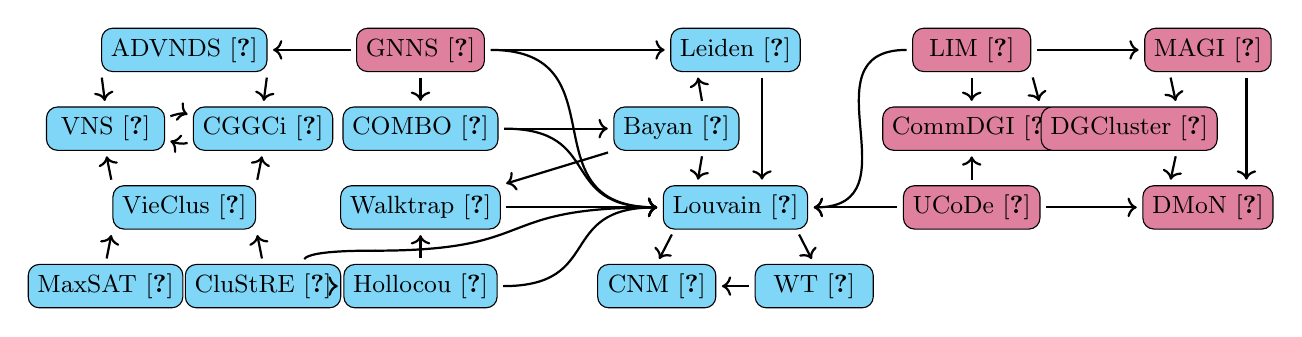
\begin{tikzpicture}[
            paper/.style={
                    draw,
                    rectangle,
                    rounded corners,
                    align=left,
                    font=\small,
                    minimum width=1.5cm,
                    minimum height=0.5cm
                },
            cite/.style={
                    ->,
                    thick,
                    shorten >=2pt,
                    shorten <=2pt
                },
            ae/.style={
                    fill=cyan!50
                },
            ml/.style={
                    fill=purple!50
                },
            node distance=0.3cm
        ]

        \node[paper, ae] (advnds) at (1, 5) {ADVNDS~\cite{advnds2019}};
        \node[paper, ae] (vns) at (0, 4) {VNS~\cite{vns2012}};
        \node[paper, ae] (cggci) at (2, 4) {CGGCi~\cite{vns2012}};
        \node[paper, ae] (vieclus) at (1, 3) {VieClus~\cite{vieclus2018}};
        \node[paper, ae] (maxsat) at (0, 2) {MaxSAT~\cite{maxsat2025}};
        \node[paper, ae] (clustre) at (2, 2) {CluStRE~\cite{clustre2025}};
        \node[paper, ml] (gnns) at (4, 5) {GNNS~\cite{gnns2022}};
        \node[paper, ae] (combo) at (4, 4) {COMBO~\cite{combo2014}};
        \node[paper, ae] (walktrap) at (4, 3) {Walktrap~\cite{walktrap2005}};
        \node[paper, ae] (hollocou) at (4, 2) {Hollocou~\cite{hollocou2017}};
        \node[paper, ae] (leiden) at (8, 5) {Leiden~\cite{leiden2019}};
        \node[paper, ae] (bayan) at (7.25, 4) {Bayan~\cite{bayan2024}};
        \node[paper, ae] (louvain) at (8, 3) {Louvain~\cite{louvain2008}};
        \node[paper, ae] (cnm) at (7, 2) {CNM~\cite{cnm2004}};
        \node[paper, ae] (wt) at (9, 2) {WT~\cite{wt2007}};
        \node[paper, ml] (lim) at (11, 5) {LIM~\cite{lim2025}};
        \node[paper, ml] (commdgi) at (11, 4) {CommDGI~\cite{commdgi2020}};
        \node[paper, ml] (ucode) at (11, 3) {UCoDe~\cite{ucode2023}};
        \node[paper, ml] (dgcluster) at (13, 4) {DGCluster~\cite{dgcluster2024}};
        \node[paper, ml] (magi) at (14, 5) {MAGI~\cite{magi2024}};
        \node[paper, ml] (dmon) at (14, 3) {DMoN~\cite{dmon2023}};

        % GNNS
        \draw[cite] (gnns.east) to[out=0, in=180, looseness=1.5] (louvain.west);
        \draw[cite] (gnns.west) to (advnds.east);
        \draw[cite] (gnns.east) to (leiden.west);
        \draw[cite] (gnns.south) to (combo.north);

        % COMBO
        \draw[cite] (combo.east) to[out=0, in=180, looseness=1.5] (louvain.west);
        \draw[cite] (combo.east) to (bayan.west);

        % Leiden
        \draw[cite] (leiden.-40) to (louvain.40);

        % Bayan
        \draw[cite] (bayan.-40) to (louvain.150);
        \draw[cite] (bayan.40) to (leiden.-150);
        \draw[cite] (bayan.south west) to (walktrap.north east);

        % Walktrap
        \draw[cite] (walktrap) to (louvain);

        % Hollocou
        \draw[cite] (hollocou.east) to[out=0, in=180, looseness=1.5] (louvain.west);
        \draw[cite] (hollocou.north) to (walktrap.south);

        % UCoDe
        \draw[cite] (ucode.west) to (louvain.east);
        \draw[cite] (ucode.north) to (commdgi.south);
        \draw[cite] (ucode.east) to (dmon.west);

        % LIM
        \draw[cite] (lim.west) to[out=180, in=0, looseness=1.5] (louvain.east);
        \draw[cite] (lim.south) to (commdgi.north);
        \draw[cite] (lim.east) to (magi.west);
        \draw[cite] (lim.south east) to (dgcluster.north west);

        % MAGI
        \draw[cite] (magi.-150) to (dgcluster.25);
        \draw[cite] (magi.-30) to (dmon.30);

        % DGCluster
        \draw[cite] (dgcluster.-25) to (dmon.150);

        % CluStRE
        \draw[cite, -] (clustre.30) to[out=60, in=180, looseness=0.5] (3.5, 2.45);
        \draw[cite] (3.35, 2.45) to[out=0, in=180, looseness=1.5] (louvain.west);
        \draw[cite] (clustre.north) to (vieclus.south east);
        \draw[cite] (clustre.east) to (hollocou.west);

        % Louvain
        \draw[cite] (louvain.-160) to (cnm.north);
        \draw[cite] (louvain.-20) to (wt.north);

        % WT
        \draw[cite] (wt.west) to (cnm.east);

        % MaxSAT
        \draw[cite] (maxsat.north) to (vieclus.south west);

        % VieClus
        \draw[cite] (vieclus.north east) to (cggci.south);
        \draw[cite] (vieclus.north west) to (vns.south);

        % ADVCNDS
        \draw[cite] (advnds.south east) to (cggci.north);
        \draw[cite] (advnds.south west) to (vns.north);

        % VNS
        \draw[cite] (vns.10) to[out=20, in=160] (cggci.170);

        % CGGCi
        \draw[cite] (cggci.190) to[out=200, in=-20] (vns.-10);

    \end{tikzpicture}

    % Normal caption
    \caption{Previous experimental comparisons visualized. Each directed edge indicates that the source algorithm used the destination algorithm in the experimental evaluation. The colors indicate either a learning-based method when red, or a classical optimization algorithm when blue.}
    % Description for someone who can't see (only clear text)
    \Description{Test.}
    \label{fig:comparisons}
\end{figure*}
We review objective functions and algorithmic paradigms for community detection and introduce the taxonomy used in this work.

Many clustering quality measures have been proposed, including \emph{coverage}, \emph{performance}~\cite{Gaertler2005}, \emph{inter-cluster conductance}~\cite{kannan2004clusterings}, \emph{surprise}~\cite{arnau2004iterative}, and \emph{modularity}~\cite{girvan2002}. Coverage, the fraction of intra-cluster edges, is simple but favors trivial solutions. Modularity mitigates this by comparing observed coverage to its expectation under a null model, and has become one of the most widely used objectives for community detection~\cite{licommunitydetectionsurvey24}. It is the primary quality function in large-scale benchmarks such as the DIMACS challenges~\cite{dimacschallengegraphpartandcluster} and is the focus of this work. While Aref et al.~\cite{survey2023} report that modularity heuristics rarely attain optimal solutions, Ans{'o}tegui et al.~\cite{maxsat2025} show that the \textsc{VieClus}'s modularity maximization heuristic routinely computes optimal solutions on small to medium-sized graphs.
%A well-known limitation in modularity is the resolution limit~\cite{resolution2007},which can cause small but well-defined communities to be merged into larger ones. Many modularity-based algorithms provide a \textsc{resolution} parameter to detect smaller communities in large graphs~\cite{louvain2008, leiden2019}. 
Alternative objectives capture complementary notions of community structure: \textit{Weighted Community Cluster} (WCC) maximizes the number of triangles within each community~\cite{wcc2012}, implemented in the  \textsc{Scalable Community Detection} algorithm~\cite{scd2014}, and the \textit{Map Equation}, which measures the expected description length of a random walk~\cite{infomap2008}, used in \textsc{Infomap}~\cite{infomap2008}, \textsc{Infoflow}~\cite{infoflow2019}, and the recent learning-based \textsc{Neuromap}~\cite{neuromap2024}. We do not include all the methods based on alternative objective functions in order to maintain our focus on modularity maximization.

Classical modularity-based algorithms use discrete optimization heuristics that consider graph topology only. More recently, learning-based approaches to community detection have been proposed, motivated by the development of GNNs that can model node attributes as feature vectors to capture additional graph information beyond topology alone. 
These methods typically optimize training objectives that are explicitly aligned with modularity or related structural principles.
Compared to classical heuristics, learning-based methods trade exact modularity gains for flexibility, the ability to incorporate node attributes, and increased generalization across graphs.
Despite extensive work in both paradigms, existing surveys do not provide a unified experimental comparison of classical and learning-based modularity optimization methods. Prior surveys typically focus on either classical heuristics~\cite{survey2023} or learning-based methods~\cite{Liu2020,Jin2023,liang2024,Messias2025}.
Li et al.~\cite{Li2024} compare classical and deep learning methods, but limit comparison to Python-based solvers, thus lacking a comprehensive comparison of the state-of-the-art. In addition, algorithmic papers in both paradigms rarely evaluate against methods outside their own class (see Figure~\ref{fig:comparisons}).

\begin{table}
    \caption{Comparison of benchmarked methods. \textit{Code} indicates implementation availability ($\times$: unavailable; $\star$: available but not ready for use; $\star\star$: open source with well-defined I/O). \textit{Features} indicate parallelism (P), automatic or user-specified number of clusters (A/K), learning-based methods (L), use of node features (F), and availability in portable Python packages (Py). The bold methods are exact solvers.}
    \label{tab:comp}
    \vspace{-0.7em}
    % \begin{tabular}{rrrrrrrrrr}
    %     \toprule
    %     Method    & Year & Code Available    & Stochastic & Parallel   & Learning-Based & Features   & Fixed $|C|$ & Exact      & Approx. Running Time      \\
    %     \midrule
    %     CNM       & 2004 & $\star\star\star$ &            &            &                &            &             &            & $\mathcal{O}(n\log^2{}n)$ \\
    %     Walktrap  & 2005 & $\star\star\star$ & \checkmark &            &                &            &             &            & $\mathcal{O}(n^2\log{}n)$ \\
    %     WT        & 2007 & $\star\star\star$ &            &            &                &            &             &            & Improved CNM              \\
    %     Louvain   & 2008 & $\star\star\star$ & \checkmark &            &                &            &             &            & ?                         \\
    %     CGGCI     & 2012 & $\times$          & ?          &            &                &            &             &            & ?                         \\
    %     VNS       & 2012 & $\times$          & \checkmark &            &                &            &             &            & ?                         \\
    %     COMBO     & 2014 & $\star\star\star$ & \checkmark &            &                &            &             &            & ?                         \\
    %     ADVNDS    & 2017 & $\times$          & \checkmark &            &                &            &             &            & Search-based              \\
    %     Hollocou  & 2017 & $\star\star$      & ?          &            &                &            &             &            & ?                         \\
    %     VieClus   & 2018 & $\star\star$      & \checkmark & \checkmark &                &            &             &            & ?                         \\
    %     Leiden    & 2019 & $\star\star\star$ & \checkmark & \checkmark &                &            &             &            & ?                         \\
    %     DMoN      & 2020 & $\star$           & \checkmark & \checkmark & \checkmark     & \checkmark & \checkmark  &            & ?                         \\
    %     CommDGI   & 2020 & $\star$           & \checkmark & \checkmark & \checkmark     & \checkmark & \checkmark  &            & ?                         \\
    %     GNNS      & 2022 & $\star$           & \checkmark & \checkmark & \checkmark     &            &             &            & ?                         \\
    %     UCoDe     & 2023 & $\star$           & \checkmark & \checkmark & \checkmark     & \checkmark & \checkmark  &            & ?                         \\
    %     DGCluster & 2023 & $\star$           & \checkmark & \checkmark & \checkmark     & \checkmark &             &            & ?                         \\
    %     MAGI      & 2024 & $\star$           & \checkmark & \checkmark & \checkmark     & \checkmark & \checkmark  &            & ?                         \\
    %     Bayan     & 2024 & $\star\star$      &            &            &                &            &             & \checkmark & ?                         \\
    %     CluStRE   & 2025 & $\star\star$      & ?          &            &                &            &             &            & ?                         \\
    %     LIM       & 2025 & $\star$           & \checkmark & \checkmark & \checkmark     & \checkmark &             &            & ?                         \\
    %     MaxSAT    & 2025 & $\times$          &            &            &                &            &             & \checkmark & ?                         \\
    %     \bottomrule
    % \end{tabular}
    \begin{tabular}{lrrlp{2cm}}
        \toprule
        Method                                     & Year & Code         &                      & Features            \\
        \midrule
        \textsc{CNM}~\cite{cnm2004}                & 2004 & $\star\star$ & \cite{cdlib2019}     & \texttt{. A . . Py} \\
        \textsc{Walktrap}~\cite{walktrap2005}      & 2005 & $\star\star$ & \cite{igraph2006}    & \texttt{. A . . Py} \\
        \textsc{WT}~\cite{wt2007}                  & 2007 & $\star\star$ & \cite{igraph2006}    & \texttt{. A . . Py} \\
        \textsc{Louvain}~\cite{louvain2008}        & 2008 & $\star\star$ & \cite{igraph2006}    & \texttt{. A . . Py} \\
        \textsc{CGGCI}~\cite{cggci_rg2012}         & 2012 & $\times$     &                      & \texttt{. A . . .}  \\
        \textsc{VNS}~\cite{vns2012}                & 2012 & $\times$     &                      & \texttt{. A . . .}  \\
        \textsc{COMBO}~\cite{combo2014}            & 2014 & $\star\star$ & \cite{comboRepo}     & \texttt{. A . . Py} \\
        \textsc{ADVNDS}~\cite{advnds2019}          & 2017 & $\times$     &                      & \texttt{. A . . .}  \\
        \textsc{Hollocou}~\cite{hollocou2017}      & 2017 & $\star\star$ & \cite{hollocouRepo}  & \texttt{. A . . .}  \\
        \textsc{VieClus}~\cite{vieclus2018}        & 2018 & $\star\star$ & \cite{vieclusRepo}   & \texttt{P A . . Py}  \\
        \textsc{Leiden}~\cite{leiden2019}          & 2019 & $\star\star$ & \cite{igraph2006}    & \texttt{. A . . Py} \\
        \textsc{DMoN}~\cite{dmon2023}              & 2020 & $\star$      & \cite{dmonRepo}      & \texttt{P K L F .}  \\
        \textsc{CommDGI}~\cite{commdgi2020}        & 2020 & $\star$      & \cite{commdgiRepo}   & \texttt{P K L F .}  \\
        \textsc{GNNS}~\cite{gnns2022}              & 2022 & $\star$      & \cite{gnnsRepo}      & \texttt{P A L . .}  \\
        \textsc{UCoDe}~\cite{ucode2023}            & 2023 & $\star$      & \cite{ucodeRepo}     & \texttt{P K L F .}  \\
        \textsc{DGCluster}~\cite{dgcluster2024}    & 2023 & $\star$      & \cite{dgclusterRepo} & \texttt{P A L F .}  \\
        \textsc{MAGI}~\cite{magi2024}              & 2024 & $\star$      & \cite{magiRepo}      & \texttt{P K L F .}  \\
        \textbf{\textsc{Bayan}}~\cite{bayan2024}   & 2024 & $\star\star$ & \cite{bayanRepo}     & \texttt{. A . . .}  \\
        \textsc{CluStRE}~\cite{clustre2025}        & 2025 & $\star\star$ & \cite{clustreRepo}   & \texttt{. A . . .}  \\
        \textsc{LIM}~\cite{lim2025}                & 2025 & $\star$      & \cite{limRepo}       & \texttt{P A L F .}  \\
        \textbf{\textsc{MaxSAT}}~\cite{maxsat2025} & 2025 & $\times$     &                      & \texttt{. A . . .}  \\
        \bottomrule
    \end{tabular}
\end{table}

%First,  The main motivation for this survey, and reason for focusing primarily on modularity optimization, is highlighted in Figure~\ref{fig:comparisons}. Despite high interest from multiple scientific communities and the rapid development of new methods, comparisons between methods remain fragmented. This is a problem for both practitioners who want the best algorithm and for future researchers who need to decide which baseline algorithms to use.

This work addresses this gap by providing a comprehensive experimental comparison of modularity-based community detection algorithms under a unified framework. Here, we provide a taxonomy of the considered methods listed in Table~\ref{tab:comp}. We organize methods by \emph{optimization paradigm}, distinguishing between \emph{classical} combinatorial algorithms and \emph{learning-based} approaches with trainable parameters. Classical methods are further grouped by their dominant optimization mechanism (e.g., greedy, multilevel, or metaheuristic) and by computational setting (e.g., streaming and exact solvers). Learning-based methods are categorized by how modularity is used during training, separating approaches that directly optimize continuous relaxations of modularity from those that use modularity as a guiding signal within broader learning objectives. 
Within each subgroup, algorithms are listed chronologically.

\subsection{Classical Modularity Optimization Methods}

\subsubsection{Greedy agglomeration and multilevel local search}

Early approaches to modularity maximization focused on greedy agglomeration, merging communities to directly increase modularity.
Subsequent work identified limitations of purely agglomerative strategies, notably unbalanced merges and poor scalability, shifting toward multilevel formulations based on local vertex moves.

\textbf{Clauset--Newman--Moore (\textsc{CNM})}~\cite{cnm2004} is a hierarchical agglomerative algorithm that greedily maximizes modularity.
Starting from singleton communities (each vertex assigned to its own cluster), it repeatedly merges the pair of communities with the largest modularity gain.
The algorithm produces a dendrogram representing the full merge hierarchy and returns the clustering attaining maximum modularity. Its running time is $O(md \log n)$, where $d$ is the dendrogram depth.

\textbf{Wakita--Tsurumi (\textsc{WT})}~\cite{wt2007} refines \textsc{CNM} by addressing its tendency to produce highly unbalanced merges that degrade scalability on large graphs.
While preserving the same agglomerative structure, \textsc{WT} modifies merge selection to account for both modularity gain and a community-size ratio, biasing the process toward more balanced agglomerations and improving scalability.

\textbf{\textsc{Louvain}}~\cite{louvain2008} replaces community-pair merging with greedy local vertex moves.
Vertices are iteratively moved to neighboring communities whenever the induced modularity gain is positive.
Once no improving move exists, communities are contracted into supernodes and the process is repeated, yielding a multilevel optimization scheme.
Each local-moving phase runs in time linear in the number of edges, and the number of multilevel passes is typically small, resulting in near-linear runtime in practice.

\textbf{\textsc{Leiden}}~\cite{leiden2019} addresses \textsc{Louvain}'s tendency to produce disconnected communities by introducing a refinement phase before contraction.
This phase splits and restructures communities through probabilistic, non-greedy merges, while guaranteeing that resulting communities are connected and locally optimal.

\subsubsection{Non-modularity baselines}

We include two widely used non-modularity baselines which rely on random walks to model how information or flow propagates through the network, providing an alternative perspective to modularity optimization.

\textbf{\textsc{WalkTrap}}~\cite{walktrap2005} performs hierarchical clustering based on the intuition that random walks on a graph tend to get "trapped" into densely connected regions corresponding to communities. 
Each vertex is characterized by the probability distribution over vertices reached by a random walk starting from it, and a structural similarity distance between vertices (and communities) is defined by comparing these distributions. Communities are then obtained by agglomerative merging of the closest pairs under this distance, producing a dendrogram similar to \textsc{CNM}. The algorithm runs in $O(m n d)$ time, where $d$ is the depth of the resulting dendrogram.

\textbf{\textsc{Infomap}}~\cite{infomap2008} formulates community detection as an information-theoretic problem, seeking a clustering that minimizes the expected description length of a random walk under the map equation.
It uses a \textsc{Louvain} inspired greedy multilevel search, augmented with fine- and coarse-tuning steps to escape local minima like \textsc{Leiden}.

\subsubsection{Metaheuristics and ensemble/hybrid search}

Beyond greedy and multilevel heuristics, several methods apply metaheuristic or ensemble-learning strategies to modularity maximization.
Representative examples include Variable Neighborhood Search (\textsc{VNS})~\cite{vns2012}, which systematically perturbs the current clustering to escape local optima, and ensemble-based approaches such as \textsc{CGGCi-RG}~\cite{cggci_rg2012}, which stabilize modularity optimization by consolidating recurring community structures across multiple runs.
These methods combine diversification mechanisms (e.g., randomized perturbations or multiple initializations) with intensification via modularity-based local refinement.
While more computationally expensive than purely greedy algorithms, such strategies often achieve higher modularity by exploring a larger search space.

\textbf{\textsc{COMBO}}~\cite{combo2014} considers pairs of communities and evaluates full redistributions of vertices between them using Kernighan--Lin–style refinements, instead of relocating individual vertices as in \textsc{Louvain}.
By unifying merges, splits, and partial recombinations, \textsc{COMBO} can escape local optima that trap multilevel greedy methods, at the cost of higher computational complexity. The algorithm runs in $O(n^2 C)$ time, where $C$ is the number of clusters.

\textbf{\textsc{VieClus}}~\cite{vieclus2018} further extends ensemble-based optimization by adopting a memetic (evolutionary) framework.
Rather than refining a single partition, it maintains a population of clusterings and generates new solutions through recombination and mutation.
Recombination exploits agreement between high-quality solutions via overlay clustering, where two vertices are grouped together only if they co-occur in both parent solutions, while mutation introduces controlled perturbations to preserve diversity.
Each offspring is refined using \textsc{Louvain} or multilevel local search and retained only if it improves modularity. After a set time limit, \textsc{VieClus} returns the best clustering found thus far. 

\subsubsection{Streaming algorithms}

Most classical modularity algorithms assume random access to the full graph, which becomes infeasible for large or dynamically generated networks.
Streaming algorithms address this limitation by processing the graph incrementally under strict memory constraints, typically allowing only a single or few passes over the data.

\textbf{\textsc{Hollocou}}~\cite{hollocou2017} is a one-pass edge-streaming algorithm.
The algorithm starts from the singleton clustering and processes edges sequentially.
For an arriving edge $(u,v)$, \textsc{Hollocou} decides whether to merge the communities of $u$ and $v$ based on their current community volumes.
If both volumes are below a fixed threshold, the node belonging to the smaller-volume community joins the other.
The authors show that under random stream orderings, this local, volume-based merging rule corresponds to a greedy optimization of modularity in the streaming setting.

\textbf{\textsc{CluStRE}}~\cite{clustre2025} follows the node-streaming model unlike the edge-streaming model of \textsc{Hollocou}. Here, nodes arrive sequentially together with their neighborhood lists.
Starting from singleton clustering, each node is assigned to the cluster among its neighbors that maximizes the modularity gain similar to a \textsc{Louvain} local move.
During streaming, a quotient graph is constructed whose nodes represent clusters and whose weighted edges summarize inter- and intra-cluster connectivity, preserving modularity exactly.
This quotient graph is optionally refined using \textsc{VieClus}.
The graph may be re-streamed to perform further improvements until convergence.

\subsubsection{Exact solvers}

In contrast to heuristic approaches, exact algorithms provably compute globally optimal modularity clusters.
Since modularity maximization is NP-hard~\cite{Brandes2008}, these methods rely on exponential-time search augmented with bounding techniques or logical formulations such as weighted partial MaxSAT~\cite{maxsat2025}, and are therefore limited to small or medium-sized graphs.

\textbf{\textsc{Bayan}}~\cite{bayan2024} is an exact branch-and-cut algorithm for modularity maximization.
It formulates modularity as an integer program with binary co-membership variables and enforces consistency via triangular constraints on node triples, which branch on whether three nodes must belong to the same community or cannot all be clustered together.
Upper bounds are obtained by solving linear programming relaxations, while lower bounds are computed from feasible clusterings produced by \textsc{COMBO}.
Branching decisions either contract node triples into supernodes or discourage their co-assignment, and the algorithm terminates once optimality is certified or a prescribed optimality gap is reached.

\subsection{Learning-Based Methods}

\subsubsection{Continuous and differentiable modularity maximization}\hfill

\noindent These approaches replace discrete community assignments with continuous representations, often learned using GNNs, expressing modularity as a continuous or differentiable objective optimized over node representations or soft cluster assignments.

\textbf{\textsc{DMoN}}~\cite{dmon2023} introduces a differentiable relaxation of modularity and realizes it using a GNN.
A GNN followed by a softmax function produces soft cluster assignments, which are optimized using an objective whose main term corresponds to modularity in spectral form. 
The objective further includes a \emph{collapse regularization} term that prevents trivial solutions in which all nodes are assigned to the same cluster.

\textbf{\textsc{GNNS}}~\cite{gnns2022} formulates modularity maximization as a continuous optimization process over soft cluster assignments.
Starting from random assignments, node assignments are iteratively updated by combining previous assignments with modularity-weighted aggregation of neighboring assignments.
Activation functions and normalization steps amplify valid assignments supported by positive modularity contributions.
The procedure is repeated for multiple random initializations and parameter choices, and the best converged solution is discretized to obtain the final clustering.

Most learning-based modularity methods, including \textsc{DMoN}, require the number of communities to be specified a priori. \textbf{\textsc{DGCluster}}~\cite{dgcluster2024} eliminates this requirement by learning node embeddings with a GNN and clustering implicitly through a joint optimization objective.
Node embeddings learned by a GNN induce soft pairwise community assignments, which parameterize a differentiable modularity objective.
A secondary loss incorporates auxiliary local information, such as partial labels or clusterings from classical heuristics, by aligning embedding similarities with a pairwise similarity matrix.
After end-to-end optimization, final communities are obtained by clustering the learned embeddings using \textsc{BIRCH}~\cite{birch1996}.

While \textsc{DGCluster} removes the need to predefine the number of communities, it relies on jointly optimizing multiple objectives which increases model and training complexity.
\textbf{\textsc{LIM}}~\cite{lim2025} addresses this trade-off with a single-objective formulation that still does not require prior specification of the number of communities.
The method first applies \textsc{Louvain} to extract coarse global communities, which are summarized as structural community centers in a feature space.
A graph convolutional network then learns node representations that capture local structural information and node attributes.
Soft cluster assignments are computed by measuring similarity between node representations and the structural centers, and a single modularity objective defined over these assignments is optimized to obtain the final clustering.

\subsubsection{Contrastive/infomax objectives}

These methods do not optimize modularity directly, but instead use it to guide representation learning through alternative objectives.

\textbf{Community Deep Graph Infomax (\textsc{CommDGI})}~\cite{commdgi2020} learns community-aware node representations by jointly maximizing mutual information between nodes and the graph and between nodes and their communities.
Unlike other methods that directly optimize modularity, modularity is used here as an auxiliary objective together with mutual information, via a soft $k$-means–style clustering layer, to encourage structurally coherent communities.

\textbf{Unified Community Detection (\textsc{UCoDe})}~\cite{ucode2023} optimizes a single contrastive objective derived from the modularity matrix, encouraging high similarity within communities and low similarity across communities.
This contrastive formulation allows \textsc{UCoDe} to recover non-overlapping communities while naturally supporting overlap, without requiring separate objectives or post-processing.
Compared to combined-objective methods such as \textsc{CommDGI}, \textsc{UCoDe} uses a single, interpretable loss and requires minimal hyperparameter tuning.

\textbf{\textsc{MAGI}}~\cite{magi2024} establishes a formal connection between modularity maximization and graph contrastive learning by showing that modularity naturally defines positive and negative node pairs via the sign of the modularity matrix.
Specifically, node pairs with positive modularity coefficients are treated as positive samples, while pairs with non-positive coefficients are treated as negatives, yielding a contrastive objective equivalent to relaxed modularity maximization.
A GNN encoder is trained using a community-aware contrastive loss, with mini-batch modularity matrices constructed via random-walk sampling for scalability.

\section{Evaluation Framework}\label{sec:evaluation}
In this section, we describe the benchmarking methodology used to evaluate modularity-based graph clustering algorithms under controlled and reproducible conditions. A central contribution is the integration of 17 clustering algorithms behind a unified benchmarking interface, offering a fair comparison across diverse implementations. In addition to enabling the experiments presented in this survey, it will also serve as an openly available resource for future work on graph clustering, simplifying the evaluation of older methods on new data or machines. This section also includes details on the datasets we used to evaluate the clustering algorithms.

\subsection{Benchmarking Interface}

As shown in Table~\ref{tab:comp}, over half of the clustering algorithms in the literature lack ready-to-use interfaces for clustering new data. Furthermore, among those with properly documented code, there are wide differences in the input graph format, output formats, and the additional information they report, such as time and memory consumption. This lack of standardization complicates fair benchmarking, as differences in preprocessing, reporting, and resource accounting can substantially affect observed performance.

To address this problem, we aim to provide an interface with a single common input and output format and consistent time and memory monitoring. The interface exposes a common set of inputs, while allowing solver-specific parameters to be provided when applicable:
\[\textsc{Cluster}(G, T_{\max}, p, k, M_{\max}, \mathcal{F})\]
where $G$ is the input graph, $T_{\max}$ is the wall-clock time limit, $p$ is the number of threads available to the algorithm, $k$ is the number of clusters to compute, $M_{\max}$ is the memory limit in gigabytes, and~$\mathcal{F}$ are the graph features. Parameters $p$, $k$, and~$\mathcal{F}$ are only used by a subset of the solvers. From Table~\ref{tab:comp}, parallel solvers use $p$, those that compute a fixed number of clusters use $k$, and any solver that uses graph features can optionally accept $\mathcal{F}$. When $\mathcal{F}$ is not provided, but the solver expects features, a single 1.0 value is assigned to each vertex as the feature. This interface is designed to capture the most common operational requirements across clustering algorithms while enforcing consistent resource limits and output reporting.

%Regarding code changes, we have tried to make as few modifications to the original source code as possible.
Whenever possible, we use the authors' implementations or the most commonly used library implementation. The exact setup for each algorithm is described in our openly available GitHub repository\footnote{\url{https://github.com/ClusterBenchmark/ClusterBenchmark}}. We make only minimal, deliberate modifications where necessary to ensure consistent timing, memory accounting, and output quality measures based on the following rules:

\begin{itemize}
    \item Parsing the input and writing the output to a file is not counted in the timing of the algorithm.
    \item For search-based algorithms that always run for the entire $T_{\max}$ duration, the recorded computation time is defined as the point in time when the best solution is found.
    \item Learning-based methods that train a neural network as part of the algorithm will break the training loop at $T_{\max}$, and use the current model at that time to produce \hbox{the final clustering.}
\end{itemize}

\subsection{Parameter Settings}

Where possible, we use the default configurations for all algorithms. Here, we detail the exact parameters chosen for each algorithm. Algorithms that are not listed do not expose any parameters.

\paragraph*{\textbf{Parameter selection policy.}}
To reflect how algorithms are typically used in practice, we deliberately avoid any dataset-specific or instance-specific parameter tuning. Our goal is to benchmark available implementations as they are, rather than hypothetical optimal configurations that would require extensive tuning effort.

\begin{itemize}
    \item \textsc{Walktrap}: walk length $=4$.
    \item \textsc{Louvain}: resolution $=1$.
    \item \textsc{Hollocou}: $v_{\max}=10\,000$.
    \item \textsc{VieClus}: time limit $=1$ hour.
    \item \textsc{Leiden}: resolution $=1$, $\beta=0.02$, iterations $=2$.
    \item \textsc{DMoN}: 1 hidden layer (64), $1\,000$ epochs, lr $=0.001$.
    \item \textsc{CommDGI}: 1 hidden layer (512), $1\,000$ epochs, lr $=0.001$.
    \item \textsc{GNNS}: \textsc{GNNS100} variant.
    \item \textsc{UCoDe}: 2 hidden layers (256), $1\,000$ epochs, lr $=0.001$.
    \item \textsc{DGCluster}: hidden layers (256, 128), 300 epochs, lr $=0.001$.
    \item \textsc{MAGI}: hidden layers (512, 256), 100 epochs, lr $=0.01$.
    \item \textsc{Bayan}: Gurobi ILP solver~\cite{gurobi}, gap $=10^{-4}$, resolution $=1$.
    \item \textsc{CluStRE}: light mode, modularity objective.
    \item \textsc{LIM}: 1 hidden layer (512), $1\,000$ epochs, patience $=200$, \hbox{lr $=0.001$.}
\end{itemize}

For stochastic algorithms with an explicitly specified seed, we use the run ID as the seed for each of the five runs. While many of these algorithms include multiple configurations, we use either the configuration recommended by the authors or the default configuration provided with the implementation.

\subsection{Dataset}

We consider three datasets commonly used in the literature. The first set consists of 10 real-world graphs with known community labels; we refer to this dataset as the \textsc{Ground-Truth} graphs. The machine learning algorithms commonly use these graphs, and the details of the instances are shown in Table~\ref{tab:ground_truth_graphs}. Next, we consider the instances used in the 10th DIMACS implementation challenge on graph clustering~\cite{dimacschallengegraphpartandcluster}; we call this dataset \textsc{DIMACS} graphs. This dataset is popular among the classical modularity optimization methods, and the details of these graphs are shown in Appendix~\ref{sec:instances}. Finally, we use synthetically generated graphs with node features generated using the attributed, degree-corrected stochastic block model (ADC-SBM)~\cite{adcsbm2022}. This generator plants $k$ clusters in the graph, and generates random edges via a distribution that is conditional on those clusters. It does so using the two input parameters $d$ and $d_{out} \leq d$, where $d$ is the expected degree for each vertex and $d_{out}$ is the expected number of neighbors for a node in a different cluster than its own. The ADC-SBM generator also produces node features that are correlated with the community structure. It does so using the two input parameters $\sigma$ for intra-cluster center variance and $\sigma_c$ for cluster center variance.

\begin{table}
    \caption{\textsc{Ground-Truth} graphs. The $|C|$ column shows the number of clusters and $x$ the number of features.}
    \label{tab:ground_truth_graphs}
    \vspace{-0.7em}
    \begin{tabular}{lrrrr}
        \toprule
        Instance         & $n$                & $m$                 & $x$ & $|C|$         \\
        \midrule
        Cora             & \numprint{2708}    & \numprint{5278}     & \numprint{1433} & \numprint{7}  \\
        Citeseer         & \numprint{3327}    & \numprint{4552}     & \numprint{3703} & \numprint{6}  \\
        Amazon-Photo     & \numprint{7650}    & \numprint{119081}   & \numprint{745}  & \numprint{8}  \\
        Amazon-Computers & \numprint{13752}   & \numprint{245861}   & \numprint{767}  & \numprint{10} \\
        Coauthor-CS      & \numprint{18333}   & \numprint{81894}    & \numprint{6805} & \numprint{15} \\
        Pubmed           & \numprint{19717}   & \numprint{44324}    & \numprint{500}  & \numprint{3}  \\
        Coauthor-Physics & \numprint{34493}   & \numprint{247962}   & \numprint{8415} & \numprint{5}  \\
        ogbn-Arxiv       & \numprint{169343}  & \numprint{1157799}  & \numprint{128}  & \numprint{40} \\
        Reddit           & \numprint{232965}  & \numprint{57307946} & \numprint{602}  & \numprint{41} \\
        ogbn-Products    & \numprint{2449029} & \numprint{61859012} & \numprint{100}  & \numprint{47} \\
        \bottomrule
    \end{tabular}
    \vspace{-1em}
\end{table}

\section{Experiments}\label{sec:experiments}
\pgfplotsset{
cycle list/.define={my marks}{
every mark/.append style={solid,fill=\pgfkeysvalueof{/pgfplots/mark list fill}},mark=*\\
every mark/.append style={solid,fill=\pgfkeysvalueof{/pgfplots/mark list fill}},mark=square*\\
every mark/.append style={solid,fill=\pgfkeysvalueof{/pgfplots/mark list fill}},mark=triangle*\\
every mark/.append style={solid,fill=\pgfkeysvalueof{/pgfplots/mark list fill}},mark=diamond*\\
every mark/.append style={solid,fill=\pgfkeysvalueof{/pgfplots/mark list fill}},mark=halfcircle*\\
every mark/.append style={solid,fill=\pgfkeysvalueof{/pgfplots/mark list fill}, mark options={rotate=90}, scale=1.25},mark=halfsquare right*\\
every mark/.append style={solid,fill=\pgfkeysvalueof{/pgfplots/mark list fill}},mark=triangle*\\
every mark/.append style={solid,fill=\pgfkeysvalueof{/pgfplots/mark list fill}},mark=halfdiamond*\\
every mark/.append style={solid,fill=\pgfkeysvalueof{/pgfplots/mark list fill}},mark=10-pointed star\\
},
perf/.style={
        ymin=0, ymax=1, xmax=1, xmin=0.0,
        axis lines=middle,
        axis x line*=bottom,
        axis y line*=left,
        cycle list/Dark2,
        cycle multiindex* list={
                my marks\nextlist
                Dark2\nextlist
                linestyles\nextlist
            },
        mark list fill={.!75!white},
        tick label style={font=\footnotesize},
        x dir=reverse,
        x axis line style={-},
        y axis line style={-}
    }
}

\begin{figure*}[!ht]

    \begin{tikzpicture}
        \begin{groupplot}[
                group style={
                        group size=4 by 1,
                        horizontal sep=0cm
                    },
                height=0.3\textwidth,
                perf,
                legend style={
                        draw=none,
                        legend columns=8,
                        legend cell align=left
                    }
            ]

            \nextgroupplot[
                width=0.35\textwidth,
                xmin=0.92,
                ylabel near ticks,
                ylabel={Fraction of instances},
                title={\textsc{Ground-Truth} Set -- F1 Scores},
                title style={xshift=1.5cm, yshift=0.06cm}
            ]

            \foreach \alg in {vieclus,leiden,louvain,combo,gnns,wt,cnm,walktrap,commdgi,clustre_fast,dmon,lim,hollocou,magi,dgcluster,ucode}{
                    \addplot+[] table[x={\alg}, y=fraction, col sep=comma] {data/real_world_perf.csv};
                    \label{\alg}
                }

            \nextgroupplot[
                width=0.25\textwidth,
                xmax=0.9,
                yticklabels=\empty,
                xtick={0.6, 0.3, 0.0},
                xlabel={$\tau$}
            ]

            \foreach \alg in {vieclus,leiden,louvain,combo,gnns,wt,cnm,walktrap,commdgi,clustre_fast,dmon,lim,hollocou,magi,dgcluster,ucode}{
                    \addplot+[] table[x={\alg}, y=fraction, col sep=comma] {data/real_world_perf.csv};
                }

            \nextgroupplot[
                xshift=1.5cm,
                width=0.25\textwidth,
                xmin=0.90,
                xtick={1.0, 0.95, 0.90},
                ylabel near ticks,
                ylabel={Fraction of instances},
                title={\textsc{DIMACS} Set -- Modularity},
                title style={xshift=2cm}
            ]

            \foreach \alg in {vieclus,leiden,louvain,combo,gnns,wt,cnm,walktrap,commdgi,clustre_fast,dmon,lim,hollocou,magi,dgcluster,ucode}{
                    \addplot+[] table[x={\alg}, y=fraction, col sep=comma] {data/dimacs_perf.csv};
                }

            \nextgroupplot[
                legend to name=sharedlegend,
                width=0.35\textwidth,
                xmax=0.90,
                yticklabels=\empty,
                xtick={0.8, 0.6, 0.4, 0.2, 0.0},
                xlabel={$\tau$}
            ]

            \foreach \alg in {vieclus,leiden,louvain,combo,gnns,wt,cnm,walktrap,commdgi,clustre_fast,dmon,lim,hollocou,magi,dgcluster,ucode}{
                    \addplot+[] table[x={\alg}, y=fraction, col sep=comma] {data/dimacs_perf.csv};
                }

            \addlegendentry{VieClus}
            \addlegendentry{Leiden}
            \addlegendentry{Louvain}
            \addlegendentry{COMBO}
            \addlegendentry{GNNS}
            \addlegendentry{WT}
            \addlegendentry{CNM}
            \addlegendentry{Walktrap}
            \addlegendentry{CommDGI}
            \addlegendentry{CluStRE}
            \addlegendentry{DMoN}
            \addlegendentry{LIM}
            \addlegendentry{Hollocou}
            \addlegendentry{MAGI}
            \addlegendentry{DGCluster}
            \addlegendentry{UCoDe}

        \end{groupplot}
    \end{tikzpicture}

    \ref{sharedlegend}

    \vspace{-0.7em}
    % Normal caption
    \caption{Performance profiles for our first two datasets. We use F1 scores for the \textsc{Ground-Truth} set and modularity for the \textsc{DIMACS} instances. For clarity, we split the x-axis to highlight the differences between the best algorithms near one. }
    % Description for someone who can't see (only clear text)
    \Description{Test.}
    \label{fig:perf_quality}
    \vspace{-1em}
\end{figure*}

In this section, we present benchmark results obtained using the unified benchmarking interface described in Section~\ref{sec:evaluation}. We report results on real-world graphs with and without ground-truth labels, as well as on synthetically generated graphs with controlled structural and feature noise. Rather than exhaustively ranking algorithms, these experiments illustrate how different algorithmic design choices behave under a standardized benchmarking setup. To support this, we also provide a dynamic website reporting updated results\footnote{\url{https://clusterbenchmark.github.io/}}.

\subsection{Computational Environment}

All algorithms are evaluated on the same machine to eliminate variability due to hardware differences and ensure fair comparison. While some methods could potentially benefit from specialized accelerators such as GPUs, we intentionally restrict all experiments to a shared CPU-based environment to maintain consistency across algorithms. We use a machine with an AMD EPYC 9754 128-core processor with 755 GB of memory, running Ubuntu 24.04.3 with Linux kernel 6.8.0-87. For algorithms with compiled software, we use GCC version 13.3.0, and for Python implementations we use Python version 3.12.3.

To accelerate the overall benchmarking process, we evaluate up to three algorithm instances concurrently on the same machine. This level of concurrency is deliberately conservative relative to the available hardware: the system provides 128 CPU cores and 755~GB of memory, ensuring substantial resource headroom for each run and minimizing contention effects. In particular, we observed that a single process cannot saturate memory bandwidth on this platform, making cross-talk between concurrently evaluated algorithms negligible in practice. Algorithms that support parallel execution internally are evaluated with 16 threads. We also record results using a single thread to test scalability. Each algorithm–instance pair is subject to a wall-clock time limit of one hour and a memory limit of 250~GB. Runs exceeding the memory limit are terminated and recorded as \emph{memory limit exceeded} (MLE). Time limits are enforced more leniently, as several learning-based methods train for a fixed number of iterations rather than converging to a stopping criterion; only runs exceeding the time limit by more than 50\% are terminated and recorded as \emph{time limit exceeded} (TLE).

For algorithms requiring a prescribed number of clusters, we provide the ground-truth value when available and set $k=16$ otherwise, following common practice. For stochastic methods, we report the best result over five independent runs. In addition to modularity (Section~\ref{sec:preliminary}), we evaluate clustering quality using Normalized Mutual Information (NMI) and an edge-restricted pairwise F1 score. The NMI score measures the level of agreement between the predicted clusters and the ground-truth clusters. For more detailed information, refer to Danon et al.~\cite{danon2005comparing}. The F1 score is computed over adjacent vertex pairs: an edge $(u,v)$ is a true positive (TP) if $u$ and $v$ are assigned to the same cluster by the algorithm as well as in the ground-truth clusters. Similarly, we define false positives (FP), true negatives (TN), and false negatives (FN). The F1 score is then calculated using the formula:  $F1 := \frac{2TP}{2TP + FP + FN}$.

\paragraph*{\textbf{Performance profiles}}

Performance profiles are well-suited for benchmarking multiple algorithms, as they summarize relative performance across instances without requiring direct aggregation of objective values~\cite{perf2002}. A performance profile assigns each algorithm a non-decreasing, piecewise-constant function. The y-axis represents the fraction of graphs where the objective value is better than or equal to $\tau$ times the best observed objective value from any algorithm. Reading a performance profile, an algorithm performs well if it achieves lower $\tau$ values for higher fractions of instances.

\subsection{State-of-the-Art Comparisons}

Figure~\ref{fig:perf_quality} shows the main results of the experimental comparison. Across both datasets, \textsc{VieClus} achieves the highest modularity whenever it completes within the imposed resource limits, consistent with prior findings~\cite{vieclus2018,maxsat2025}. As expected for a memetic search-based method, it exceeds the memory limit on the two largest \hbox{DIMACS instances.}

On the \textsc{Ground-Truth} dataset, many methods achieve similarly high F1 scores. Among them, \textsc{MAGI} achieves the strongest and most stable performance. This highlights a general mismatch between modularity optimization and externally defined communities. For example, the Citeseer ground-truth clustering has a modularity of 0.54, whereas all methods produce clusterings with modularity above 0.54. This discrepancy reflects the fact that citation behavior does not necessarily align with categorical labels, as Figure~\ref{fig:comparisons} \hbox{also indicates.}

For the \textsc{DIMACS} graphs, differences between methods are more pronounced, with modularity-focused algorithms clearly outperforming learning-based approaches. Among learning-based methods, performance varies substantially depending on whether the method is designed to operate without node features, with \textsc{GNNS} performing best in this setting.

The streaming methods \textsc{Hollocou} and \textsc{CluStRE} trade solution quality for extreme efficiency. While their F1 scores are lower on the \textsc{Ground-Truth} dataset, \textsc{CluStRE} achieves competitive modularity on DIMACS instances while using orders of magnitude less time and memory. The exact algorithm \textsc{Bayan} terminates only on the eight smallest instances from the \textsc{DIMACS} dataset and is therefore excluded from the performance profiles. For these graphs, \textsc{VieClus} found the optimal clustering for all of them, \textsc{Leiden} for 7/8, \textsc{GNNS} for 5/8, \textsc{COMBO} for 4/8, and \textsc{Louvain} for 3/8. The remaining algorithms did not find any known optimal solutions.

\pgfplotsset{
cycle list/.define={my marks}{
every mark/.append style={solid,fill=\pgfkeysvalueof{/pgfplots/mark list fill}},mark=*\\
every mark/.append style={solid,fill=\pgfkeysvalueof{/pgfplots/mark list fill}},mark=square*\\
every mark/.append style={solid,fill=\pgfkeysvalueof{/pgfplots/mark list fill}},mark=triangle*\\
every mark/.append style={solid,fill=\pgfkeysvalueof{/pgfplots/mark list fill}},mark=diamond*\\
every mark/.append style={solid,fill=\pgfkeysvalueof{/pgfplots/mark list fill}},mark=halfcircle*\\
every mark/.append style={solid,fill=\pgfkeysvalueof{/pgfplots/mark list fill}, mark options={rotate=90}, scale=1.25},mark=halfsquare right*\\
every mark/.append style={solid,fill=\pgfkeysvalueof{/pgfplots/mark list fill}},mark=triangle*\\
every mark/.append style={solid,fill=\pgfkeysvalueof{/pgfplots/mark list fill}},mark=halfdiamond*\\
every mark/.append style={solid,fill=\pgfkeysvalueof{/pgfplots/mark list fill}},mark=10-pointed star\\
},
perf/.style={
        ymin=0, ymax=1,
        axis lines=middle,
        axis x line*=bottom,
        axis y line*=left,
        cycle list/Dark2,
        cycle multiindex* list={
                my marks\nextlist
                Dark2\nextlist
                linestyles\nextlist
            },
        mark list fill={.!75!white},
        tick label style={font=\footnotesize},
        x axis line style={-},
        y axis line style={-}
    }
}

\begin{figure*}[!ht]

    \begin{tikzpicture}
        \begin{groupplot}[
                group style={
                        group size=2 by 1,
                        horizontal sep=1.5cm
                    },
                height=0.25\textwidth,
                width=0.5\textwidth,
                perf,
                legend style={
                        draw=none,
                        legend columns=6,
                        legend cell align=left
                    }
            ]

            \nextgroupplot[xmax=14, xmin=1.0,
                xlabel=$d_{out}$,
                xlabel style={xshift=-2.4cm},
                ylabel=NMI,
                ylabel near ticks]

            \foreach \alg in {vieclus,dmon,commdgi,ucode,dgcluster,magi}{
                    \expanded{
                        \noexpand\addplot+ [refstyle={\alg}] table[x=dout, y={\alg}, col sep=comma] {data/dout_data.csv};
                    }
                }

            \nextgroupplot[xmode=log, legend to name=sharedlegend2,
                xlabel=$\sigma_c$,
                ylabel=NMI,
                ylabel near ticks]

            \foreach \alg in {vieclus,dmon,commdgi,ucode,dgcluster,magi}{
                    \expanded{
                        \noexpand\addplot+ [refstyle={\alg}] table[x=sigma, y={\alg}, col sep=comma] {data/sigma_data.csv};
                    }
                }

            \addlegendentry{VieClus}
            \addlegendentry{DMoN}
            \addlegendentry{CommDGI}
            \addlegendentry{UCoDe}
            \addlegendentry{DGCluster}
            \addlegendentry{MAGI}

        \end{groupplot}
    \end{tikzpicture}

    % \vspace{0.5em}
    \ref{sharedlegend2}

    % Normal caption
    \vspace{-0.7em}
    \caption{ NMI scores on graphs generated with the ADC-SBM graph generator. All graphs have $n=\numprint{1000}$ vertices, $k=4$ clusters, $d=20$ average degree, and $\sigma=1$ intra-cluster center variance. The left plot varies $d_{out}$ while keeping $\sigma_c=3$, and the right plot varies $\sigma_c$ while keeping $d_{out}=2$. }
    % Description for someone who can't see (only clear text)
    \Description{Test.}
    \label{fig:adcsbm}
    \vspace{-1em}
\end{figure*}

\pgfplotsset{
cycle list/.define={my marks}{
every mark/.append style={solid,fill=\pgfkeysvalueof{/pgfplots/mark list fill}},mark=*\\
every mark/.append style={solid,fill=\pgfkeysvalueof{/pgfplots/mark list fill}},mark=square*\\
every mark/.append style={solid,fill=\pgfkeysvalueof{/pgfplots/mark list fill}},mark=triangle*\\
every mark/.append style={solid,fill=\pgfkeysvalueof{/pgfplots/mark list fill}},mark=diamond*\\
every mark/.append style={solid,fill=\pgfkeysvalueof{/pgfplots/mark list fill}},mark=halfcircle*\\
every mark/.append style={solid,fill=\pgfkeysvalueof{/pgfplots/mark list fill}, mark options={rotate=90}, scale=1.25},mark=halfsquare right*\\
every mark/.append style={solid,fill=\pgfkeysvalueof{/pgfplots/mark list fill}},mark=triangle*\\
every mark/.append style={solid,fill=\pgfkeysvalueof{/pgfplots/mark list fill}},mark=halfdiamond*\\
every mark/.append style={solid,fill=\pgfkeysvalueof{/pgfplots/mark list fill}},mark=10-pointed star\\
}
}

\begin{figure}[!h]

    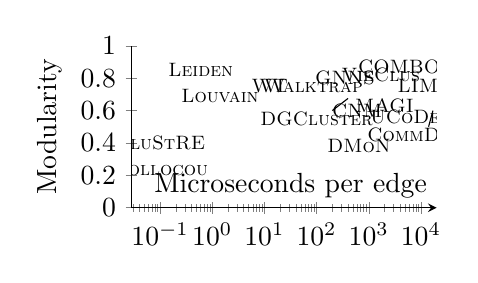
\begin{tikzpicture}
        \begin{axis}[
                ymin=0.0, ymax=1.0,
                height=0.3\textwidth,
                width=0.45\textwidth,
                xmax=20000,
                xmode=log,
                axis lines=middle,
                axis x line*=bottom,
                axis y line*=left,
                y axis line style={-},
                cycle list/Dark2,
                cycle multiindex* list={
                        my marks\nextlist
                        Dark2\nextlist
                        linestyles\nextlist
                    },
                mark size=3pt,
                ylabel near ticks,
                ylabel={Modularity},
                xlabel={Microseconds per edge},
                legend style={
                        draw=none,
                        legend columns=4,,
                        legend cell align=left,
                        at={(-0.2,-0.7)}, anchor=south west
                    }
            ]

            \addplot[refstyle={vieclus}] coordinates {(1726.3660110940255,0.7531085752527071)};
            \node at (1700, 0.82) {\scriptsize \textsc{VieClus}};

            \addplot[refstyle={leiden}] coordinates {(0.6239696880930304,0.7621314735947818)};
            \node at (0.6, 0.85) {\scriptsize \textsc{Leiden}};

            \addplot[refstyle={louvain}] coordinates {(1.4013229432695928,0.7547851126538677)};
            \node at (1.4, 0.69) {\scriptsize \textsc{Louvain}};

            \addplot[refstyle={combo}] coordinates {(2820.7939174904686,0.766180333291874)};
            \node at (3820, 0.87) {\scriptsize \textsc{COMBO}};

            \addplot[refstyle={gnns}] coordinates {(559.3278503834495,0.7178744368397761)};
            \node at (350, 0.8) {\scriptsize \textsc{GNNS}};

            \addplot[refstyle={wt}] coordinates {(12.771122157737215,0.6642441446299415)};
            \node at (12.7, 0.75) {\scriptsize \textsc{WT}};

            \addplot[refstyle={cnm}] coordinates {(660.5783649792988,0.6758815349295846)};
            \node at (600, 0.6) {\scriptsize \textsc{CNM}};

            \addplot[refstyle={walktrap}] coordinates {(86.36169664105313,0.6727992787112209)};
            \node at (86.4, 0.75) {\scriptsize \textsc{Walktrap}};

            \addplot[refstyle={commdgi}] coordinates {(19499.523710563695, 0.6603309780162184)};
            \node at (8000, 0.45) {\scriptsize \textsc{CommDGI}};
            \draw (14000, 0.5) -- (17000, 0.6);

            \addplot[refstyle={clustre_fast}] coordinates {(0.08779015323918948,0.49019129511178766)};
            \node at (0.1, 0.4) {\scriptsize \textsc{CluStRE}};

            \addplot[refstyle={dmon}] coordinates {(648.5178048996712,0.45727461117777635)};
            \node at (648, 0.38) {\scriptsize \textsc{DMoN}};

            \addplot[refstyle={lim}] coordinates {(8692.783865262756,0.6680899707353964)};
            \node at (8700, 0.75) {\scriptsize \textsc{LIM}};

            \addplot[refstyle={hollocou}] coordinates {(0.02831508257184716,0.2385322144468167)};
            \node at (0.1, 0.238) {\scriptsize \textsc{Hollocou}};

            \addplot[refstyle={magi}] coordinates {(3564.7727114111008,0.6850822252894211)};
            \node at (2000, 0.63) {\scriptsize \textsc{MAGI}};

            \addplot[refstyle={dgcluster}] coordinates {(600.0758423676813,0.713305998339106)};
            \node at (100, 0.55) {\scriptsize \textsc{DGCluster}};
            \draw (200, 0.6) -- (400, 0.675);

            \addplot[refstyle={ucode}] coordinates {(5577.320249077159,0.6202928248036939)};
            \node at (5000, 0.56) {\scriptsize \textsc{UCoDe}};


            % \addlegendentry{VieClus}
            % \addlegendentry{Leiden}
            % \addlegendentry{Louvain}
            % \addlegendentry{COMBO}
            % \addlegendentry{GNNS}
            % \addlegendentry{WT}
            % \addlegendentry{CNM}
            % \addlegendentry{Walktrap}
            % \addlegendentry{CommDGI}
            % \addlegendentry{CluStRE}
            % \addlegendentry{DMoN}
            % \addlegendentry{LIM}
            % \addlegendentry{Hollocou}
            % \addlegendentry{MAGI}
            % \addlegendentry{DGCluster}
            % \addlegendentry{UCoDe}

        \end{axis}
    \end{tikzpicture}

    % Normal caption
    \vspace{-0.7em}
    \caption{ Scatter plot showing the ratio between running time and solution quality, using the geometric mean for both measures on the \textsc{Ground-Truth} graphs. To normalize the running time per graph, we divide it by the number of edges, yielding a time-per-edge measure. }
    % Description for someone who can't see (only clear text)
    \Description{Test.}
    \label{fig:efficiency}
    \vspace{-1em}
\end{figure}

\subsection{Quality--Efficiency Tradeoffs}

Figure~\ref{fig:efficiency} summarizes the tradeoff between clustering quality and execution time using geometric means across instances. Streaming methods occupy the extreme low-latency regime, while greedy modularity methods (\textsc{Louvain}, \textsc{Leiden}) achieve a favorable balance between quality and efficiency. The search-based algorithm \textsc{VieClus} achieves the highest quality, but at a substantially higher computational cost. Similarly, learning-based methods generally attain high solution qualities at substantially higher \hbox{computational cost.}

Peak memory usage varies significantly across methods, and detailed measurements for the \textsc{Ground-Truth} dataset are presented in Appendix~\ref{sec:memory}. This appendix also offers insights into the number of training iterations completed by each learning-based algorithm. Although the largest instances often face memory or time constraints, most algorithms complete all training iterations, showing that GPUs or other accelerators would not have improved the results for those smaller graphs. We also evaluate the parallel algorithms sequentially to analyze how additional computing resources affect their performance; detailed measurements are presented \hbox{in Appendix~\ref{sec:par-seq}.}

% \subfile{../tables/memory.tex}

\subsection{Synthetic Graphs}

To further evaluate the impact and sensitivity of graph features across clustering algorithms, we include experiments with syntactically generated graphs with vertex features. These experiments illustrate how feature-aware methods respond to controlled degradation of structural and attribute signals, rather than ranking the methods. For reference, we also include \textsc{VieClus}, which performed best among the pure modularity-optimizing methods. We conduct two sets of experiments with the ADC-SBM generator. First, we generate a sequence of graphs with gradually higher $d_{out}$, causing the graph structure to carry less information about the original $k$ clusters. And second, we generate graphs with strong community structure as we gradually increase the cluster center variance $\sigma_c$, leading the graph features to carry less information \hbox{about the clusters.}

Figure~\ref{fig:adcsbm} summarizes the results of the two ADC-SBM experiments. When the feature signal is strong, \textsc{MAGI} and \textsc{DMoN} achieve the highest NMI scores, and beyond $d_{out} \approx 11$, all feature-aware methods outperform \textsc{VieClus}. The results also highlight clear differences in how methods balance structural and feature information. \textsc{MAGI} relies primarily on node features, as evidenced by its strong performance under structural noise and its sensitivity to feature degradation. In contrast, \textsc{DMoN} remains robust in both settings, indicating a more balanced use of topology and attributes. \textsc{CommDGI} exhibits similar trends but performs consistently worse than \textsc{DMoN}. \textsc{DGCluster} shows the opposite bias to \textsc{MAGI}, favoring graph structure over features, while \textsc{UCoDe} displays a similar but less pronounced tendency. We exclude \textsc{LIM} from this figure, as it consistently collapsed to a single cluster, yielding zero NMI across all configurations.

\section{Conclusion}\label{sec:conclusion}
We surveyed 17 modularity-based graph clustering algorithms, covering classical heuristics, parallel methods, and recent learning-based approaches. When modularity maximization is the sole objective, the results are clear: \textsc{VieClus} consistently achieves the highest modularity values when sufficient memory is available. \textsc{Leiden}, an improved variant of \textsc{Louvain}, closely follows in solution quality and offers substantially faster runtimes. This trade-off reflects their optimization strategies: \textsc{VieClus} relies on time-budgeted search, while \textsc{Leiden} uses a greedy refinement scheme.

Beyond modularity alone, other algorithms exhibit their own unique strengths. Streaming methods such as \textsc{CluStRE} offer extremely low runtimes and memory footprints, making them well-suited for large-scale or resource-constrained settings. Learning-based approaches, including \textsc{GNNS}, demonstrate that neural methods are approaching the performance of hand-crafted heuristics. However, they still require substantially more memory and do not yet achieve competitive modularity scores. At the same time, there is growing interest in expanding modularity optimization with auxiliary objectives to recover ground-truth communities better. In this setting, feature-aware methods can be advantageous: \textsc{MAGI} achieves the strongest ground-truth recovery in our experiments, while \textsc{DMoN} remains effective when community structure is encoded between topology and node attributes.

To support future work in this area, we introduce a unified benchmarking framework that enables direct, reproducible comparisons across a wide range of modularity-based clustering algorithms. We hope that this framework lowers the barrier for evaluating new methods against established baselines and encourages more systematic experimental studies of graph clustering algorithms.

\section*{Acknowledgements}
We acknowledge support by DFG grant SCHU 2567/5-1.

\section*{Author Contributions}
A.C., K.L., and C.S. conceived the study. K.L. and A.C. developed the benchmark framework, performed the experiments, and analyzed the data. K.L., A.C., and C.S. wrote the manuscript.

\section*{Competing Interests}
The authors declare no competing interests.

\section*{Data and Code Availability}
The complete benchmarking harness, solver wrappers, and datasets are open-source and publicly available at \url{https://github.com/TODO/ClusterBenchmark}.

\begin{thebibliography}{10}
\expandafter\ifx\csname url\endcsname\relax
  \def\url#1{\texttt{#1}}\fi
\expandafter\ifx\csname urlprefix\endcsname\relax\def\urlprefix{URL }\fi
\providecommand{\bibinfo}[2]{#2}
\providecommand{\eprint}[2][]{\url{#2}}

\bibitem{Newman2003}
\bibinfo{author}{Newman, M. E.~J.}
\newblock \bibinfo{title}{Properties of highly clustered networks}.
\newblock \emph{\bibinfo{journal}{Phys. Rev. E}} \textbf{\bibinfo{volume}{68}},
  \bibinfo{pages}{026121} (\bibinfo{year}{2003}).
\newblock \urlprefix\url{https://link.aps.org/doi/10.1103/PhysRevE.68.026121}.

\bibitem{McFarling89}
\bibinfo{author}{McFarling, S.}
\newblock \bibinfo{title}{Program optimization for instruction caches}.
\newblock In \bibinfo{editor}{Emer, J.~S.} \& \bibinfo{editor}{Hennessy, J.~L.}
  (eds.) \emph{\bibinfo{booktitle}{{ASPLOS-III} Proceedings - Third
  International Conference on Architectural Support for Programming Languages
  and Operating Systems, Boston, Massachusetts, USA, April 3-6, 1989}},
  \bibinfo{pages}{183--191} (\bibinfo{publisher}{{ACM} Press},
  \bibinfo{year}{1989}).
\newblock \urlprefix\url{https://doi.org/10.1145/70082.68200}.

\bibitem{Demme2012}
\bibinfo{author}{Demme, J.} \& \bibinfo{author}{Sethumadhavan, S.}
\newblock \bibinfo{title}{Approximate graph clustering for program
  characterization}.
\newblock \emph{\bibinfo{journal}{{ACM} Trans. Archit. Code Optim.}}
  \textbf{\bibinfo{volume}{8}}, \bibinfo{pages}{21:1--21:21}
  (\bibinfo{year}{2012}).
\newblock \urlprefix\url{https://doi.org/10.1145/2086696.2086700}.

\bibitem{Akoglu2015}
\bibinfo{author}{Akoglu, L.}, \bibinfo{author}{Tong, H.} \&
  \bibinfo{author}{Koutra, D.}
\newblock \bibinfo{title}{Graph based anomaly detection and description: a
  survey}.
\newblock \emph{\bibinfo{journal}{Data Min. Knowl. Discov.}}
  \textbf{\bibinfo{volume}{29}}, \bibinfo{pages}{626--688}
  (\bibinfo{year}{2015}).
\newblock \urlprefix\url{https://doi.org/10.1007/s10618-014-0365-y}.

\bibitem{Xu2002}
\bibinfo{author}{Xu, Y.}, \bibinfo{author}{Olman, V.} \& \bibinfo{author}{Xu,
  D.}
\newblock \bibinfo{title}{Clustering gene expression data using a
  graph-theoretic approach: an application of minimum spanning trees}.
\newblock \emph{\bibinfo{journal}{Bioinform.}} \textbf{\bibinfo{volume}{18}},
  \bibinfo{pages}{536--545} (\bibinfo{year}{2002}).
\newblock \urlprefix\url{https://doi.org/10.1093/bioinformatics/18.4.536}.

\bibitem{Cai2011}
\bibinfo{author}{Cai, B.}, \bibinfo{author}{Wang, H.}, \bibinfo{author}{Zheng,
  H.} \& \bibinfo{author}{Wang, H.}
\newblock \bibinfo{title}{Detection of functional modules from protein
  interaction networks with an enhanced random walk based algorithm}.
\newblock \emph{\bibinfo{journal}{Int. J. Comput. Biol. Drug Des.}}
  \textbf{\bibinfo{volume}{4}}, \bibinfo{pages}{290--306}
  (\bibinfo{year}{2011}).
\newblock \urlprefix\url{https://doi.org/10.1504/IJCBDD.2011.041416}.

\bibitem{Newman2006}
\bibinfo{author}{Newman, M. E.~J.}
\newblock \bibinfo{title}{Modularity and community structure in networks}.
\newblock \emph{\bibinfo{journal}{Proceedings of the National Academy of
  Sciences}} \textbf{\bibinfo{volume}{103}}, \bibinfo{pages}{8577--8582}
  (\bibinfo{year}{2006}).
\newblock \urlprefix\url{https://www.pnas.org/doi/abs/10.1073/pnas.0601602103}.
\newblock \eprint{https://www.pnas.org/doi/pdf/10.1073/pnas.0601602103}.

\bibitem{Brandes2008}
\bibinfo{author}{Brandes, U.} \emph{et~al.}
\newblock \bibinfo{title}{On modularity clustering}.
\newblock \emph{\bibinfo{journal}{{IEEE} Trans. Knowl. Data Eng.}}
  \textbf{\bibinfo{volume}{20}}, \bibinfo{pages}{172--188}
  (\bibinfo{year}{2008}).
\newblock \urlprefix\url{https://doi.org/10.1109/TKDE.2007.190689}.

\bibitem{girvan2002}
\bibinfo{author}{Girvan, M.} \& \bibinfo{author}{Newman, M. E.~J.}
\newblock \bibinfo{title}{Community structure in social and biological
  networks}.
\newblock \emph{\bibinfo{journal}{Proceedings of the National Academy of
  Sciences}} \textbf{\bibinfo{volume}{99}}, \bibinfo{pages}{7821--7826}
  (\bibinfo{year}{2002}).
\newblock \urlprefix\url{https://www.pnas.org/doi/abs/10.1073/pnas.122653799}.
\newblock \eprint{https://www.pnas.org/doi/pdf/10.1073/pnas.122653799}.

\bibitem{cnm2004}
\bibinfo{author}{Clauset, A.}, \bibinfo{author}{Newman, M. E.~J.} \&
  \bibinfo{author}{Moore, C.}
\newblock \bibinfo{title}{Finding community structure in very large networks}.
\newblock \emph{\bibinfo{journal}{Physical Review E}}
  \textbf{\bibinfo{volume}{70}}, \bibinfo{pages}{066111}
  (\bibinfo{year}{2004}).

\bibitem{walktrap2005}
\bibinfo{author}{Pons, P.} \& \bibinfo{author}{Latapy, M.}
\newblock \bibinfo{title}{Computing communities in large networks using random
  walks}.
\newblock In \emph{\bibinfo{booktitle}{Proceedings of the 20th International
  Symposium on Computer and Information Sciences (ISCIS 2005)}},
  \bibinfo{pages}{284--293} (\bibinfo{publisher}{Springer Berlin Heidelberg},
  \bibinfo{year}{2005}).

\bibitem{wt2007}
\bibinfo{author}{Wakita, K.} \& \bibinfo{author}{Tsurumi, T.}
\newblock \bibinfo{title}{Finding community structure in mega-scale social
  networks: [extended abstract]}.
\newblock In \emph{\bibinfo{booktitle}{Proceedings of the 16th International
  Conference on World Wide Web (WWW 2007)}}, \bibinfo{pages}{1275--1276}
  (\bibinfo{publisher}{Association for Computing Machinery},
  \bibinfo{year}{2007}).

\bibitem{ln2008}
\bibinfo{author}{Leicht, E.~A.} \& \bibinfo{author}{Newman, M. E.~J.}
\newblock \bibinfo{title}{Community structure in directed networks}.
\newblock \emph{\bibinfo{journal}{Physical Review Letters}}
  \textbf{\bibinfo{volume}{100}}, \bibinfo{pages}{118703}
  (\bibinfo{year}{2008}).

\bibitem{infomap2008}
\bibinfo{author}{Rosvall, M.} \& \bibinfo{author}{Bergstrom, C.~T.}
\newblock \bibinfo{title}{Maps of random walks on complex networks reveal
  community structure}.
\newblock \emph{\bibinfo{journal}{Proceedings of the National Academy of
  Sciences}} \textbf{\bibinfo{volume}{105}}, \bibinfo{pages}{1118--1123}
  (\bibinfo{year}{2008}).

\bibitem{louvain2008}
\bibinfo{author}{Blondel, V.~D.}, \bibinfo{author}{Guillaume, J.-L.},
  \bibinfo{author}{Lambiotte, R.} \& \bibinfo{author}{Lefebvre, E.}
\newblock \bibinfo{title}{Fast unfolding of communities in large networks}.
\newblock \emph{\bibinfo{journal}{Journal of Statistical Mechanics: Theory and
  Experiment}} \textbf{\bibinfo{volume}{2008}}, \bibinfo{pages}{P10008}
  (\bibinfo{year}{2008}).

\bibitem{vns2012}
\bibinfo{author}{Aloise, D.} \emph{et~al.}
\newblock \bibinfo{title}{Modularity maximization in networks by variable
  neighborhood search}.
\newblock In \emph{\bibinfo{booktitle}{Graph Partitioning and Graph
  Clustering}}, vol. \bibinfo{volume}{588} of
  \emph{\bibinfo{series}{Contemporary Mathematics}}, \bibinfo{pages}{113--127}
  (\bibinfo{publisher}{American Mathematical Society}, \bibinfo{year}{2012}).

\bibitem{cggci_rg2012}
\bibinfo{author}{Ovelg\"{o}nne, M.} \& \bibinfo{author}{Geyer-Schulz, A.}
\newblock \bibinfo{title}{An ensemble learning strategy for graph clustering}.
\newblock In \emph{\bibinfo{booktitle}{Graph Partitioning and Graph
  Clustering}}, vol. \bibinfo{volume}{588} of
  \emph{\bibinfo{series}{Contemporary Mathematics}}, \bibinfo{pages}{187--205}
  (\bibinfo{publisher}{American Mathematical Society}, \bibinfo{year}{2012}).

\bibitem{scd2014}
\bibinfo{author}{Prat-P\'{e}rez, A.}, \bibinfo{author}{Dominguez-Sal, D.} \&
  \bibinfo{author}{Larriba-Pey, J.-L.}
\newblock \bibinfo{title}{High quality, scalable and parallel community
  detection for large real graphs}.
\newblock In \emph{\bibinfo{booktitle}{Proceedings of the 23rd International
  Conference on World Wide Web (WWW 2014)}}, \bibinfo{pages}{225--236}
  (\bibinfo{publisher}{Association for Computing Machinery},
  \bibinfo{year}{2014}).

\bibitem{combo2014}
\bibinfo{author}{Sobolevsky, S.}, \bibinfo{author}{Campari, R.},
  \bibinfo{author}{Belyi, A.} \& \bibinfo{author}{Ratti, C.}
\newblock \bibinfo{title}{General optimization technique for high-quality
  community detection in complex networks}.
\newblock \emph{\bibinfo{journal}{Physical Review E}}
  \textbf{\bibinfo{volume}{90}}, \bibinfo{pages}{012811}
  (\bibinfo{year}{2014}).

\bibitem{belief2014}
\bibinfo{author}{Zhang, P.} \& \bibinfo{author}{Moore, C.}
\newblock \bibinfo{title}{Scalable detection of statistically significant
  communities and hierarchies, using message passing for modularity}.
\newblock \emph{\bibinfo{journal}{Proceedings of the National Academy of
  Sciences}} \textbf{\bibinfo{volume}{111}}, \bibinfo{pages}{18144--18149}
  (\bibinfo{year}{2014}).

\bibitem{hollocou2017}
\bibinfo{author}{Hollocou, A.}, \bibinfo{author}{Maudet, J.},
  \bibinfo{author}{Bonald, T.} \& \bibinfo{author}{Lelarge, M.}
\newblock \bibinfo{title}{A streaming algorithm for graph clustering}.
\newblock \bibinfo{howpublished}{arXiv preprint} (\bibinfo{year}{2017}).

\bibitem{vieclus2018}
\bibinfo{author}{Biedermann, S.}, \bibinfo{author}{Henzinger, M.},
  \bibinfo{author}{Schulz, C.} \& \bibinfo{author}{Schuster, B.}
\newblock \bibinfo{title}{Memetic graph clustering}.
\newblock In \emph{\bibinfo{booktitle}{Proceedings of the 17th International
  Symposium on Experimental Algorithms (SEA 2018)}}, \bibinfo{pages}{3:1--3:15}
  (\bibinfo{publisher}{Schloss Dagstuhl -- Leibniz-Zentrum f{\"u}r Informatik},
  \bibinfo{year}{2018}).

\bibitem{dane2018}
\bibinfo{author}{Gao, H.} \& \bibinfo{author}{Huang, H.}
\newblock \bibinfo{title}{Deep attributed network embedding}.
\newblock In \emph{\bibinfo{booktitle}{Proceedings of the 27th International
  Joint Conference on Artificial Intelligence (IJCAI 2018)}},
  \bibinfo{pages}{3364--3370} (\bibinfo{publisher}{International Joint
  Conferences on Artificial Intelligence Organization}, \bibinfo{year}{2018}).

\bibitem{infoflow2019}
\bibinfo{author}{Fung, P.~K.}
\newblock \bibinfo{title}{{InfoFlow}: A distributed algorithm to detect
  communities according to the map equation}.
\newblock \emph{\bibinfo{journal}{Big Data and Cognitive Computing}}
  \textbf{\bibinfo{volume}{3}}, \bibinfo{pages}{42} (\bibinfo{year}{2019}).

\bibitem{leiden2019}
\bibinfo{author}{Traag, V.~A.}, \bibinfo{author}{Waltman, L.} \&
  \bibinfo{author}{van Eck, N.~J.}
\newblock \bibinfo{title}{From {Louvain} to {Leiden}: guaranteeing
  well-connected communities}.
\newblock \emph{\bibinfo{journal}{Scientific Reports}}
  \textbf{\bibinfo{volume}{9}}, \bibinfo{pages}{5233} (\bibinfo{year}{2019}).

\bibitem{advnds2019}
\bibinfo{author}{D\v{z}ami\'{c}, D.}, \bibinfo{author}{Aloise, D.} \&
  \bibinfo{author}{Mladenovi\'{c}, N.}
\newblock \bibinfo{title}{Ascent-descent variable neighborhood decomposition
  search for community detection by modularity maximization}.
\newblock \emph{\bibinfo{journal}{Annals of Operations Research}}
  \textbf{\bibinfo{volume}{272}} (\bibinfo{year}{2019}).

\bibitem{commdgi2020}
\bibinfo{author}{Zhang, T.} \emph{et~al.}
\newblock \bibinfo{title}{{CommDGI}: Community detection oriented deep graph
  infomax}.
\newblock In \emph{\bibinfo{booktitle}{Proceedings of the 29th ACM
  International Conference on Information \& Knowledge Management (CIKM
  2020)}}, \bibinfo{pages}{1843--1852} (\bibinfo{publisher}{Association for
  Computing Machinery}, \bibinfo{year}{2020}).

\bibitem{dmon2023}
\bibinfo{author}{Tsitsulin, A.}, \bibinfo{author}{Palowitch, J.},
  \bibinfo{author}{Perozzi, B.} \& \bibinfo{author}{M\"{u}ller, E.}
\newblock \bibinfo{title}{Graph clustering with graph neural networks}.
\newblock \emph{\bibinfo{journal}{Journal of Machine Learning Research}}
  \textbf{\bibinfo{volume}{24}}, \bibinfo{pages}{1--21} (\bibinfo{year}{2023}).
\newblock \urlprefix\url{http://jmlr.org/papers/v24/20-998.html}.

\bibitem{gnns2022}
\bibinfo{author}{Sobolevsky, S.} \& \bibinfo{author}{Belyi, A.}
\newblock \bibinfo{title}{Graph neural network inspired algorithm for
  unsupervised network community detection}.
\newblock \emph{\bibinfo{journal}{Applied Network Science}}
  \textbf{\bibinfo{volume}{7}}, \bibinfo{pages}{63} (\bibinfo{year}{2022}).

\bibitem{ucode2023}
\bibinfo{author}{Moradan, A.}, \bibinfo{author}{Draganov, A.},
  \bibinfo{author}{Mottin, D.} \& \bibinfo{author}{Assent, I.}
\newblock \bibinfo{title}{{UCoDe}: Unified community detection with graph
  convolutional networks}.
\newblock \emph{\bibinfo{journal}{Machine Learning}}
  \textbf{\bibinfo{volume}{112}}, \bibinfo{pages}{5057--5080}
  (\bibinfo{year}{2023}).

\bibitem{survey2023}
\bibinfo{author}{Aref, S.}, \bibinfo{author}{Mostajabdaveh, M.} \&
  \bibinfo{author}{Chheda, H.}
\newblock \bibinfo{title}{Heuristic modularity maximization algorithms for
  community detection rarely return an optimal partition or anything similar}.
\newblock In \emph{\bibinfo{booktitle}{Proceedings of the 23th International
  Conference on Computational Science (ICCS 2023)}}, \bibinfo{pages}{612--626}
  (\bibinfo{publisher}{Springer Nature Switzerland}, \bibinfo{year}{2023}).

\bibitem{paris2024}
\bibinfo{author}{Madi, S.~A.} \& \bibinfo{author}{Pirr\`{o}, G.}
\newblock \bibinfo{title}{Node-centric community deception based on safeness}.
\newblock \emph{\bibinfo{journal}{IEEE Transactions on Computational Social
  Systems}} \textbf{\bibinfo{volume}{11}}, \bibinfo{pages}{2955--2965}
  (\bibinfo{year}{2024}).

\bibitem{dgcluster2024}
\bibinfo{author}{Bhowmick, A.}, \bibinfo{author}{Kosan, M.},
  \bibinfo{author}{Huang, Z.}, \bibinfo{author}{Singh, A.} \&
  \bibinfo{author}{Medya, S.}
\newblock \bibinfo{title}{{DGCLUSTER}: A neural framework for attributed graph
  clustering via modularity maximization}.
\newblock In \emph{\bibinfo{booktitle}{Proceedings of the 38th AAAI Conference
  on Artificial Intelligence (AAAI 2024)}}, \bibinfo{pages}{11069--11077}
  (\bibinfo{publisher}{AAAI Press, Washington, DC, USA}, \bibinfo{year}{2024}).

\bibitem{magi2024}
\bibinfo{author}{Liu, Y.} \emph{et~al.}
\newblock \bibinfo{title}{Revisiting modularity maximization for graph
  clustering: A contrastive learning perspective}.
\newblock In \emph{\bibinfo{booktitle}{Proceedings of the 30th ACM SIGKDD
  Conference on Knowledge Discovery and Data Mining (KDD 2024)}},
  \bibinfo{pages}{1968--1979} (\bibinfo{publisher}{Association for Computing
  Machinery, New York, NY, United States}, \bibinfo{year}{2024}).

\bibitem{bayan2024}
\bibinfo{author}{Aref, S.}, \bibinfo{author}{Mostajabdaveh, M.} \&
  \bibinfo{author}{Chheda, H.}
\newblock \bibinfo{title}{Bayan algorithm: Detecting communities in networks
  through exact and approximate optimization of modularity}.
\newblock \emph{\bibinfo{journal}{Physical Review E}}
  \textbf{\bibinfo{volume}{110}}, \bibinfo{pages}{044315}
  (\bibinfo{year}{2024}).

\bibitem{neuromap2024}
\bibinfo{author}{Bl{\"o}cker, C.}, \bibinfo{author}{Tan, C.} \&
  \bibinfo{author}{Scholtes, I.}
\newblock \bibinfo{title}{The map equation goes neural: Mapping network flows
  with graph neural networks}.
\newblock In \emph{\bibinfo{booktitle}{Proceedings of the 38th Conference on
  Neural Information Processing Systems (NeurIPS 2024)}},
  \bibinfo{pages}{17428--17456} (\bibinfo{publisher}{Curran Associates, Inc.},
  \bibinfo{year}{2024}).

\bibitem{clustre2025}
\bibinfo{author}{Chhabra, A.}, \bibinfo{author}{Dorian~Peretz, S.} \&
  \bibinfo{author}{Schulz, C.}
\newblock \bibinfo{title}{{CluStRE}: Streaming graph clustering with
  multi-stage refinement}.
\newblock In \emph{\bibinfo{booktitle}{Proceedings of the 23rd International
  Symposium on Experimental Algorithms (SEA 2025)}},
  \bibinfo{pages}{11:1--11:20} (\bibinfo{publisher}{Schloss Dagstuhl --
  Leibniz-Zentrum f{\"u}r Informatik}, \bibinfo{year}{2025}).

\bibitem{lim2025}
\bibinfo{author}{Wang, H.} \emph{et~al.}
\newblock \bibinfo{title}{Simple yet effective heuristic community detection
  with graph convolution network}.
\newblock \emph{\bibinfo{journal}{Scientific Reports}}
  \textbf{\bibinfo{volume}{15}}, \bibinfo{pages}{39249} (\bibinfo{year}{2025}).

\bibitem{maxsat2025}
\bibinfo{author}{Ans{\'o}tegui, C.}, \bibinfo{author}{Ramaswamy, V.~P.},
  \bibinfo{author}{Szeider, S.} \& \bibinfo{author}{Xia, H.}
\newblock \bibinfo{title}{Uncovering and verifying optimal community structure
  in complex networks: A {MaxSAT} approach}.
\newblock In \emph{\bibinfo{booktitle}{Proceedings of the 25th International
  Conference on Computational Science (ICCS 2025)}}, \bibinfo{pages}{35--49}
  (\bibinfo{publisher}{Springer Nature Switzerland}, \bibinfo{year}{2025}).

\bibitem{adcsbm2022}
\bibinfo{author}{Tsitsulin, A.}, \bibinfo{author}{Rozemberczki, B.},
  \bibinfo{author}{Palowitch, J.} \& \bibinfo{author}{Perozzi, B.}
\newblock \bibinfo{title}{Synthetic graph generation to benchmark graph
  learning}.
\newblock \bibinfo{howpublished}{arXiv preprint} (\bibinfo{year}{2022}).

\bibitem{perf2002}
\bibinfo{author}{Dolan, E.~D.} \& \bibinfo{author}{Mor\'{e}, J.~J.}
\newblock \bibinfo{title}{Benchmarking optimization software with performance
  profiles}.
\newblock \emph{\bibinfo{journal}{Mathematical Programming}}
  \textbf{\bibinfo{volume}{91}}, \bibinfo{pages}{201--213}
  (\bibinfo{year}{2002}).

\bibitem{gurobi}
\bibinfo{author}{{Gurobi Optimization, LLC}}.
\newblock \bibinfo{title}{{Gurobi Optimizer Reference Manual}}
  (\bibinfo{year}{2026}).
\newblock \urlprefix\url{https://www.gurobi.com}.

\bibitem{resolution2007}
\bibinfo{author}{Fortunato, S.} \& \bibinfo{author}{Barthelemy, M.}
\newblock \bibinfo{title}{Resolution limit in community detection}.
\newblock \emph{\bibinfo{journal}{Proceedings of the national academy of
  sciences}} \textbf{\bibinfo{volume}{104}}, \bibinfo{pages}{36--41}
  (\bibinfo{year}{2007}).

\bibitem{wcc2012}
\bibinfo{author}{Prat-P{\'e}rez, A.}, \bibinfo{author}{Dominguez-Sal, D.},
  \bibinfo{author}{Brunat, J.~M.} \& \bibinfo{author}{Larriba-Pey, J.-L.}
\newblock \bibinfo{title}{Shaping communities out of triangles}.
\newblock In \emph{\bibinfo{booktitle}{Proceedings of the 21st ACM
  international conference on Information and knowledge management}},
  \bibinfo{pages}{1677--1681} (\bibinfo{publisher}{Association for Computing
  Machinery}, \bibinfo{year}{2012}).

\bibitem{Li2024}
\bibinfo{author}{Li, J.} \emph{et~al.}
\newblock \bibinfo{title}{A comprehensive review of community detection in
  graphs}.
\newblock \emph{\bibinfo{journal}{Neurocomputing}}
  \textbf{\bibinfo{volume}{600}}, \bibinfo{pages}{128169}
  (\bibinfo{year}{2024}).
\newblock \urlprefix\url{https://doi.org/10.1016/j.neucom.2024.128169}.

\bibitem{Jin2023}
\bibinfo{author}{Jin, D.} \emph{et~al.}
\newblock \bibinfo{title}{A survey of community detection approaches: From
  statistical modeling to deep learning}.
\newblock \emph{\bibinfo{journal}{{IEEE} Trans. Knowl. Data Eng.}}
  \textbf{\bibinfo{volume}{35}}, \bibinfo{pages}{1149--1170}
  (\bibinfo{year}{2023}).
\newblock \urlprefix\url{https://doi.org/10.1109/TKDE.2021.3104155}.

\bibitem{Liu2020}
\bibinfo{author}{Liu, F.} \emph{et~al.}
\newblock \bibinfo{title}{Deep learning for community detection: Progress,
  challenges and opportunities}.
\newblock In \bibinfo{editor}{Bessiere, C.} (ed.)
  \emph{\bibinfo{booktitle}{Proceedings of the Twenty-Ninth International Joint
  Conference on Artificial Intelligence, {IJCAI} 2020}},
  \bibinfo{pages}{4981--4987} (\bibinfo{publisher}{ijcai.org},
  \bibinfo{year}{2020}).
\newblock \urlprefix\url{https://doi.org/10.24963/ijcai.2020/693}.

\bibitem{Messias2025}
\bibinfo{author}{Messias, G.~H.}, \bibinfo{author}{Gonçalves~Botelho, T.},
  \bibinfo{author}{Iasulaitis, S.}, \bibinfo{author}{Coelho~Naldi, M.} \&
  \bibinfo{author}{Demétrius Baria~Valejo, A.}
\newblock \bibinfo{title}{A systematic review of graph neural network for node
  clustering in homogeneous attributed networks}.
\newblock \emph{\bibinfo{journal}{IEEE Access}} \textbf{\bibinfo{volume}{13}},
  \bibinfo{pages}{215265--215285} (\bibinfo{year}{2025}).

\bibitem{liang2024}
\bibinfo{author}{Liang, K.} \emph{et~al.}
\newblock \bibinfo{title}{A survey of knowledge graph reasoning on graph types:
  Static, dynamic, and multi-modal}.
\newblock \emph{\bibinfo{journal}{IEEE Transactions on Pattern Analysis and
  Machine Intelligence}} \textbf{\bibinfo{volume}{46}},
  \bibinfo{pages}{9456--9478} (\bibinfo{year}{2024}).

\bibitem{Gaertler2005}
\bibinfo{author}{Gaertler, M.}
\newblock \bibinfo{title}{Clustering}.
\newblock In \bibinfo{editor}{Brandes, U.} \& \bibinfo{editor}{Erlebach, T.}
  (eds.) \emph{\bibinfo{booktitle}{Network Analysis: Methodological Foundations
  [outcome of a Dagstuhl seminar, 13-16 April 2004]}}, vol.
  \bibinfo{volume}{3418} of \emph{\bibinfo{series}{Lecture Notes in Computer
  Science}}, \bibinfo{pages}{178--215} (\bibinfo{publisher}{Springer},
  \bibinfo{year}{2004}).
\newblock \urlprefix\url{https://doi.org/10.1007/978-3-540-31955-9\_8}.

\bibitem{kannan2004clusterings}
\bibinfo{author}{Kannan, R.}, \bibinfo{author}{Vempala, S.~S.} \&
  \bibinfo{author}{Vetta, A.}
\newblock \bibinfo{title}{On clusterings: Good, bad and spectral}.
\newblock \emph{\bibinfo{journal}{J. {ACM}}} \textbf{\bibinfo{volume}{51}},
  \bibinfo{pages}{497--515} (\bibinfo{year}{2004}).
\newblock \urlprefix\url{https://doi.org/10.1145/990308.990313}.

\bibitem{arnau2004iterative}
\bibinfo{author}{Arnau, V.}, \bibinfo{author}{Mars, S.} \&
  \bibinfo{author}{Marı\'{i}n, I.}
\newblock \bibinfo{title}{{I}terative {C}luster {A}nalysis of {P}rotein
  {I}nteraction {D}ata}.
\newblock \emph{\bibinfo{journal}{Bioinformatics}}
  \textbf{\bibinfo{volume}{21}}, \bibinfo{pages}{364--378}
  (\bibinfo{year}{2004}).

\bibitem{dimacschallengegraphpartandcluster}
\bibinfo{editor}{Bader, D.~A.}, \bibinfo{editor}{Meyerhenke, H.},
  \bibinfo{editor}{Sanders, P.} \& \bibinfo{editor}{Wagner, D.} (eds.).
\newblock \emph{\bibinfo{title}{Graph Partitioning and Graph Clustering, 10th
  {DIMACS} Implementation Challenge Workshop, Georgia Institute of Technology,
  Atlanta, GA, USA, February 13-14, 2012. Proceedings}}, vol.
  \bibinfo{volume}{588} of \emph{\bibinfo{series}{Contemporary Mathematics}}
  (\bibinfo{publisher}{American Mathematical Society}, \bibinfo{year}{2013}).
\newblock \urlprefix\url{https://doi.org/10.1090/conm/588}.

\bibitem{licommunitydetectionsurvey24}
\bibinfo{author}{Li, J.} \emph{et~al.}
\newblock \bibinfo{title}{{A} {C}omprehensive {R}eview of {C}ommunity
  {D}etection in {G}raphs}.
\newblock \emph{\bibinfo{journal}{Neurocomputing}}
  \textbf{\bibinfo{volume}{600}}, \bibinfo{pages}{128169}
  (\bibinfo{year}{2024}).

\bibitem{rosvall2009map}
\bibinfo{author}{Rosvall, M.}, \bibinfo{author}{Axelsson, D.} \&
  \bibinfo{author}{Bergstrom, C.~T.}
\newblock \bibinfo{title}{{T}he {M}ap {E}quation}.
\newblock \emph{\bibinfo{journal}{The European Physical J. Special Topics}}
  \textbf{\bibinfo{volume}{178}}, \bibinfo{pages}{13--23}
  (\bibinfo{year}{2009}).

\bibitem{Peel2016}
\bibinfo{author}{Peel, L.}, \bibinfo{author}{Larremore, D.~B.} \&
  \bibinfo{author}{Clauset, A.}
\newblock \bibinfo{title}{The ground truth about metadata and community
  detection in networks}.
\newblock \emph{\bibinfo{journal}{CoRR}}
  \textbf{\bibinfo{volume}{abs/1608.05878}} (\bibinfo{year}{2016}).
\newblock \urlprefix\url{http://arxiv.org/abs/1608.05878}.
\newblock \eprint{1608.05878}.

\bibitem{Wani2024}
\bibinfo{author}{Wani, A.~A.}
\newblock \bibinfo{title}{Comprehensive analysis of clustering algorithms:
  exploring limitations and innovative solutions}.
\newblock \emph{\bibinfo{journal}{PeerJ Comput. Sci.}}
  \textbf{\bibinfo{volume}{10}}, \bibinfo{pages}{e2286} (\bibinfo{year}{2024}).
\newblock \urlprefix\url{https://doi.org/10.7717/peerj-cs.2286}.

\bibitem{10.1145/235968.233324}
\bibinfo{author}{Zhang, T.}, \bibinfo{author}{Ramakrishnan, R.} \&
  \bibinfo{author}{Livny, M.}
\newblock \bibinfo{title}{Birch: an efficient data clustering method for very
  large databases}.
\newblock \emph{\bibinfo{journal}{SIGMOD Rec.}} \textbf{\bibinfo{volume}{25}},
  \bibinfo{pages}{103–114} (\bibinfo{year}{1996}).
\newblock \urlprefix\url{https://doi.org/10.1145/235968.233324}.

\bibitem{birch1996}
\bibinfo{author}{Zhang, T.}, \bibinfo{author}{Ramakrishnan, R.} \&
  \bibinfo{author}{Livny, M.}
\newblock \bibinfo{title}{Birch: an efficient data clustering method for very
  large databases}.
\newblock In \emph{\bibinfo{booktitle}{Proceedings of the 1996 ACM SIGMOD
  International Conference on Management of Data}}, SIGMOD '96,
  \bibinfo{pages}{103–114} (\bibinfo{publisher}{Association for Computing
  Machinery}, \bibinfo{address}{New York, NY, USA}, \bibinfo{year}{1996}).
\newblock \urlprefix\url{https://doi.org/10.1145/233269.233324}.

\bibitem{cdlib2019}
\bibinfo{author}{Rossetti, G.}, \bibinfo{author}{Milli, L.} \&
  \bibinfo{author}{Cazabet, R.}
\newblock \bibinfo{title}{{CDLIB}: a python library to extract, compare and
  evaluate communities from complex networks}.
\newblock \emph{\bibinfo{journal}{Applied Network Science}}
  \textbf{\bibinfo{volume}{4}}, \bibinfo{pages}{2364--8228}
  (\bibinfo{year}{2019}).

\bibitem{igraph2006}
\bibinfo{author}{Csardi, G.} \& \bibinfo{author}{Nepusz, T.}
\newblock \bibinfo{title}{The igraph software package for complex network
  research}.
\newblock \emph{\bibinfo{journal}{InterJournal}}
  \textbf{\bibinfo{volume}{Complex Systems}}, \bibinfo{pages}{1695}
  (\bibinfo{year}{2006}).
\newblock \urlprefix\url{https://igraph.org}.

\bibitem{comboRepo}
\bibinfo{author}{Kats, P.} \& \bibinfo{author}{Belyi, A.}
\newblock \bibinfo{title}{{COMBO} repository}.
\newblock \bibinfo{howpublished}{\url{https://github.com/Casyfill/pyCombo.git}}
  (\bibinfo{year}{2026}).

\bibitem{hollocouRepo}
\bibinfo{author}{Hollocou, A.}
\newblock \bibinfo{title}{{Hollocou} repository}.
\newblock
  \bibinfo{howpublished}{\url{https://github.com/ahollocou/graph-streaming.git}}
  (\bibinfo{year}{2026}).

\bibitem{vieclusRepo}
\bibinfo{author}{Schulz, C.} \& \bibinfo{author}{Seemaier, D.}
\newblock \bibinfo{title}{{VieClus} repository}.
\newblock \bibinfo{howpublished}{\url{https://github.com/VieClus/VieClus.git}}
  (\bibinfo{year}{2026}).

\bibitem{dmonRepo}
\bibinfo{author}{Tsitsulin, A.}, \bibinfo{author}{Palowitch, J.},
  \bibinfo{author}{Perozzi, B.} \& \bibinfo{author}{M\"uller, E.}
\newblock \bibinfo{title}{{DMoN} repository}.
\newblock
  \bibinfo{howpublished}{\url{https://github.com/google-research/google-research.git}}
  (\bibinfo{year}{2026}).

\bibitem{commdgiRepo}
\bibinfo{author}{Zhang, T.} \emph{et~al.}
\newblock \bibinfo{title}{{CommDGI} repository}.
\newblock \bibinfo{howpublished}{\url{https://github.com/FDUDSDE/CommDGI.git}}
  (\bibinfo{year}{2026}).

\bibitem{gnnsRepo}
\bibinfo{author}{Belyi, A.}
\newblock \bibinfo{title}{{GNNS} repository}.
\newblock
  \bibinfo{howpublished}{\url{https://github.com/Alexander-Belyi/GNNS.git}}
  (\bibinfo{year}{2026}).

\bibitem{ucodeRepo}
\bibinfo{author}{Moradan, A.}, \bibinfo{author}{Draganov, A.},
  \bibinfo{author}{Mottin, D.} \& \bibinfo{author}{Assent, I.}
\newblock \bibinfo{title}{{UCoDe} repository}.
\newblock \bibinfo{howpublished}{\url{https://github.com/AU-DIS/UCODE.git}}
  (\bibinfo{year}{2026}).

\bibitem{dgclusterRepo}
\bibinfo{author}{Kosan, M.}
\newblock \bibinfo{title}{{DGCluster} repository}.
\newblock
  \bibinfo{howpublished}{\url{https://github.com/pyrobits/DGCluster.git}}
  (\bibinfo{year}{2026}).

\bibitem{magiRepo}
\bibinfo{author}{Li, J.}
\newblock \bibinfo{title}{{MAGI} repository}.
\newblock
  \bibinfo{howpublished}{\url{https://github.com/EdisonLeeeee/MAGI.git}}
  (\bibinfo{year}{2026}).

\bibitem{bayanRepo}
\bibinfo{author}{Mostajabdaveh, M.} \& \bibinfo{author}{Aref, S.}
\newblock \bibinfo{title}{{Bayan} repository}.
\newblock \bibinfo{howpublished}{\url{https://github.com/saref/bayan.git}}
  (\bibinfo{year}{2026}).

\bibitem{clustreRepo}
\bibinfo{author}{Chhabra, A.}
\newblock \bibinfo{title}{{CluStRE} repository}.
\newblock \bibinfo{howpublished}{\url{https://github.com/KaHIP/CluStRE.git}}
  (\bibinfo{year}{2026}).

\bibitem{limRepo}
\bibinfo{author}{Wang, H.}
\newblock \bibinfo{title}{{LIM} repository}.
\newblock
  \bibinfo{howpublished}{\url{https://github.com/wuanghoong/Less-is-More.git}}
  (\bibinfo{year}{2026}).

\bibitem{danon2005comparing}
\bibinfo{author}{Danon, L.}, \bibinfo{author}{Diaz-Guilera, A.},
  \bibinfo{author}{Duch, J.} \& \bibinfo{author}{Arenas, A.}
\newblock \bibinfo{title}{Comparing community structure identification}.
\newblock \emph{\bibinfo{journal}{Journal of Statistical Mechanics: Theory and
  Experiment}} \textbf{\bibinfo{volume}{2005}}, \bibinfo{pages}{2364--8228}
  (\bibinfo{year}{2005}).

\end{thebibliography}


\appendix

\section{Benchmark Instances}
\label{sec:instances}
\begin{table}[H]
    \caption{Graph from the 10th DIMACS implementation challange. There are no features or ground truth clusters for these graphs.}
    \label{tab:dimacs_instances}
    \begin{tabular}{lrr}
        \toprule
        Instance               & $n$                  & $m$                   \\
        \midrule
        karate                 & \numprint{34}        & \numprint{78}         \\
        chesapeake             & \numprint{39}        & \numprint{170}        \\
        dolphins               & \numprint{62}        & \numprint{159}        \\
        lesmis                 & \numprint{77}        & \numprint{254}        \\
        polbooks               & \numprint{105}       & \numprint{441}        \\
        adjnoun                & \numprint{112}       & \numprint{425}        \\
        football               & \numprint{115}       & \numprint{613}        \\
        jazz                   & \numprint{198}       & \numprint{2742}       \\
        celegansneural         & \numprint{297}       & \numprint{2148}       \\
        celegans-metabolic     & \numprint{453}       & \numprint{2025}       \\
        email                  & \numprint{1133}      & \numprint{5451}       \\
        polblogs               & \numprint{1490}      & \numprint{16715}      \\
        netscience             & \numprint{1589}      & \numprint{2742}       \\
        power                  & \numprint{4941}      & \numprint{6594}       \\
        hep-th                 & \numprint{8361}      & \numprint{15751}      \\
        PGPgiantcompo          & \numprint{10680}     & \numprint{24316}      \\
        astro-ph               & \numprint{16706}     & \numprint{121251}     \\
        cond-mat               & \numprint{16726}     & \numprint{47594}      \\
        as-22july06            & \numprint{22963}     & \numprint{48436}      \\
        cond-mat-2003          & \numprint{31163}     & \numprint{120029}     \\
        cond-mat-2005          & \numprint{40421}     & \numprint{175691}     \\
        preferentialAttachment & \numprint{100000}    & \numprint{499985}     \\
        smallworld             & \numprint{100000}    & \numprint{499998}     \\
        G-n-pin-pout           & \numprint{100000}    & \numprint{501198}     \\
        caidaRouterLevel       & \numprint{192244}    & \numprint{609066}     \\
        cnr-2000               & \numprint{325557}    & \numprint{2738969}    \\
        eu-2005                & \numprint{862664}    & \numprint{16138468}   \\
        in-2004                & \numprint{1382908}   & \numprint{13591473}   \\
        road-central           & \numprint{14081816}  & \numprint{16933413}   \\
        uk-2002                & \numprint{18520486}  & \numprint{261787258}  \\
        road-usa               & \numprint{23947347}  & \numprint{28854312}   \\
        uk-2007-05             & \numprint{105896555} & \numprint{3301876564} \\
        \bottomrule
    \end{tabular}
\end{table}

\section{Memory Usage}
\label{sec:memory}
\setlength{\tabcolsep}{4.5pt}

\begin{table}[H]
    \caption{Memory consumption of the evaluated algorithms on the \textsc{Ground-Truth} dataset. Values are reported in human-readable units. Entries marked \textsc{TLE} indicate runs exceeding the one-hour time limit, while \textsc{MLE} denotes runs exceeding the 250~GB memory limit. }
    \label{tab:memory}
    \small
    \begin{tabular}{l|rrrrrrrrrr}
        \toprule
        Method             & Cora      & Citeseer  & Amz-Photo & Amz-Comp  & CoAuth-CS & Pubmed    & CoAuth-Phys & ogbn-Arxiv & Reddit    & ogbn-Prod \\
        \midrule
        \textsc{VieClus}   & 22.53~MB  & 22.53~MB  & 64.91~MB  & 130.24~MB & 58.7~MB   & 44.94~MB  & 134.75~MB   & 497.74~MB  & 9.6~GB    & TLE       \\
        \textsc{Leiden}    & 20.48~MB  & 20.48~MB  & 38.91~MB  & 59.39~MB  & 34.82~MB  & 26.62~MB  & 61.44~MB    & 211.36~MB  & 9.01~GB   & 9.83~GB   \\
        \textsc{Louvain}   & 20.48~MB  & 20.48~MB  & 38.91~MB  & 59.39~MB  & 32.77~MB  & 28.67~MB  & 61.44~MB    & 210.32~MB  & 9.01~GB   & 9.83~GB   \\
        \textsc{COMBO}     & 255.58~MB & 314.59~MB & 1.09~GB   & 3.17~GB   & 5.42~GB   & TLE       & TLE         & MLE        & MLE       & MLE       \\
        \textsc{GNNS}      & 1.35~GB   & 1.75~GB   & 5.49~GB   & 8.1~GB    & 8.28~GB   & 8.31~GB   & 8.11~GB     & 6.09~GB    & 26.37~GB  & MLE       \\
        \textsc{WT}        & 20.48~MB  & 20.48~MB  & 38.91~MB  & 59.39~MB  & 34.82~MB  & 28.67~MB  & 61.44~MB    & 211.36~MB  & TLE       & TLE       \\
        \textsc{CNM}       & 192.51~MB & 179.96~MB & 253.07~MB & 372.06~MB & 234.14~MB & 210.71~MB & 398.65~MB   & TLE        & TLE       & TLE       \\
        \textsc{Walktrap}  & 27.32~MB  & 20.48~MB  & 418.48~MB & 1.47~GB   & 935.16~MB & 488.84~MB & 4.36~GB     & 99.06~GB   & MLE       & MLE       \\
        \textsc{CommDGI}   & 735.03~MB & 857.03~MB & 2.05~GB   & 5.34~GB   & 9.54~GB   & 9.82~GB   & 31.09~GB    & MLE        & MLE       & MLE       \\
        \textsc{CluStRE}   & 6.14~MB   & 6.14~MB   & 6.14~MB   & 6.14~MB   & 6.14~MB   & 6.14~MB   & 6.14~MB     & 8.19~MB    & 8.19~MB   & 22.53~MB  \\
        \textsc{DMoN}      & 664.01~MB & 863.31~MB & 778~MB    & 987.44~MB & 3.5~GB    & 809.3~MB  & 7.39~GB     & 735.92~MB  & 67~GB     & 77.26~GB  \\
        \textsc{LIM}       & 674.08~MB & 741.17~MB & 1.92~GB   & 4.67~GB   & 7.45~GB   & TLE       & TLE         & MLE        & MLE       & MLE       \\
        \textsc{Hollocou}  & 2.05~MB   & 2.05~MB   & 4.1~MB    & 6.14~MB   & 4.1~MB    & 4.1~MB    & 8.19~MB     & 32.39~MB   & 912.7~MB  & 1.15~GB   \\
        \textsc{MAGI}      & 807.82~MB & 992.96~MB & 1.55~GB   & 2.56~GB   & 6.15~GB   & 2.22~GB   & 15.66~GB    & TLE        & 50.74~GB  & MLE       \\
        \textsc{DGCluster} & 548.86~MB & 917.5~MB  & 879.83~MB & 1.39~GB   & 5.84~GB   & 1.07~GB   & 13.2~GB     & 624.64~MB  & 150.63~GB & TLE       \\
        \textsc{UCoDe}     & 576.89~MB & 771.56~MB & 1.7~GB    & 4.32~GB   & 7.69~GB   & 6.94~GB   & 24.23~GB    & MLE        & MLE       & MLE       \\
        \bottomrule
    \end{tabular}
\end{table}

\setlength{\tabcolsep}{4.5pt}

\begin{table}[H]
    \caption{Number of finished training iterations of the evaluated algorithms on the \textsc{Ground-Truth} dataset. Entries marked \textsc{TLE} indicate runs exceeding the one-hour time limit, while \textsc{MLE} denotes runs exceeding the 250~GB memory limit. }
    \label{tab:iterations}
    \small
    \begin{tabular}{l|rrrrrrrrrr}
        \toprule
        Method             & Cora                            & Citeseer                        & Amz-Photo                       & Amz-Comp                        & CoAuth-CS                       & Pubmed                          & CoAuth-Phys                     & ogbn-Arxiv                      & Reddit             & ogbn-Prod          \\
        \midrule
        \textsc{CommDGI}   & \numprint{1000}/\numprint{1000} & \numprint{1000}/\numprint{1000} & \numprint{1000}/\numprint{1000} & \numprint{1000}/\numprint{1000} & \numprint{628}/\numprint{1000}  & \numprint{708}/\numprint{1000}  & 224/\numprint{1000}             & MLE                             & MLE                & MLE                \\
        \textsc{DMoN}      & \numprint{1000}/\numprint{1000} & \numprint{1000}/\numprint{1000} & \numprint{1000}/\numprint{1000} & \numprint{1000}/\numprint{1000} & \numprint{1000}/\numprint{1000} & \numprint{1000}/\numprint{1000} & \numprint{1000}/\numprint{1000} & \numprint{1000}/\numprint{1000} & 24/\numprint{1000} & 17/\numprint{1000} \\
        \textsc{LIM}       & \numprint{1000}/\numprint{1000} & \numprint{1000}/\numprint{1000} & \numprint{1000}/\numprint{1000} & \numprint{874}/\numprint{1000}  & 552/\numprint{1000}             & TLE                             & TLE                             & MLE                             & MLE                & MLE                \\
        \textsc{MAGI}      & 100/100                         & 100/100                         & 100/100                         & 100/100                         & 100/100                         & 100/100                         & 31/100                          & TLE                             & 18/100             & MLE                \\
        \textsc{DGCluster} & 300/300                         & 300/300                         & 300/300                         & 300/300                         & 300/300                         & 300/300                         & 300/300                         & 300/300                         & 34/300             & TLE                \\
        \textsc{UCoDe}     & \numprint{1000}/\numprint{1000} & \numprint{1000}/\numprint{1000} & \numprint{1000}/\numprint{1000} & \numprint{1000}/\numprint{1000} & \numprint{1000}/\numprint{1000} & \numprint{1000}/\numprint{1000} & 450/\numprint{1000}             & MLE                             & MLE                & MLE                \\
        \bottomrule
    \end{tabular}
\end{table}

\section{Parallel-Sequential Comparison}
\label{sec:par-seq}
% \setlength{\tabcolsep}{7pt}

\begin{table}[H]
    \caption{Parallel and sequential running times for six instances from the \textsc{Ground-Truth} dataset. Only the parallel methods are included in the table. The $t_1$ column gives the sequential running time in seconds, while the $t_{16}$ column displays the running time with 16 threads. }
    \label{tab:par-seq}
    \small
    \begin{tabular}{l|rr|rr|rr|rr|rr|rr}
        \toprule
                           & \multicolumn{2}{c|}{Cora} & \multicolumn{2}{c|}{Citeseer} & \multicolumn{2}{c|}{Amz-Photo} & \multicolumn{2}{c|}{Amz-Comp} & \multicolumn{2}{c|}{CoAuth-CS} & \multicolumn{2}{c}{CoAuth-Phys}                                                                                                                                                                                    \\ \cline{2-13}
        Method             & \multicolumn{1}{c}{$t_1$} & \multicolumn{1}{c|}{$t_{16}$} & \multicolumn{1}{c}{$t_1$}      & \multicolumn{1}{c|}{$t_{16}$} & \multicolumn{1}{c}{$t_1$}      & \multicolumn{1}{c|}{$t_{16}$}   & \multicolumn{1}{c}{$t_1$} & \multicolumn{1}{c|}{$t_{16}$} & \multicolumn{1}{c}{$t_1$} & \multicolumn{1}{c|}{$t_{16}$} & \multicolumn{1}{c}{$t_1$} & \multicolumn{1}{c}{$t_{16}$} \\
        \midrule
        \textsc{VieClus}   & 276.55                    & 83.31                         & 8.29                           & 5.19                          & 93.29                          & 16.25                           & 2\,804.96                 & 2\,476.70                     & 2\,811.52                 & 2\,897.85                     & 3\,511.06                 & 3\,562.30                    \\
        \textsc{GNNS}      & 36.40                     & 9.41                          & 48.44                          & 11.90                         & 231.92                         & 43.46                           & 592.24                    & 115.08                        & 668.79                    & 162.44                        & 1\,906.75                 & 363.04                       \\
        \textsc{CommDGI}   & 936.72                    & 140.64                        & 2\,046.85                      & 288.34                        & 3\,606.69                      & 1\,284.26                       & 3\,616.27                 & 3\,416.34                     & 3\,613.43                 & 3\,602.34                     & 3\,664.35                 & 3\,610.59                    \\
        \textsc{DMoN}      & 55.60                     & 42.19                         & 100.31                         & 50.01                         & 312.63                         & 184.55                          & 658.25                    & 352.90                        & 868.59                    & 212.61                        & 2\,060.92                 & 498.45                       \\
        \textsc{LIM}       & 811.90                    & 97.63                         & 1\,218.18                      & 185.00                        & 3\,605.01                      & 618.07                          & 3\,614.08                 & 1\,909.42                     & 3\,633.77                 & 2\,130.90                     & TLE                       & TLE                          \\
        \textsc{MAGI}      & 119.29                    & 56.88                         & 215.38                         & 66.44                         & 1\,445.31                      & 535.17                          & 3\,605.81                 & 1\,572.78                     & 3\,635.58                 & 3\,414.73                     & 3\,691.43                 & 3\,614.21                    \\
        \textsc{DGCluster} & 44.78                     & 17.40                         & 91.01                          & 23.75                         & 301.28                         & 98.98                           & 594.48                    & 193.56                        & 833.56                    & 140.19                        & 1\,961.84                 & 307.94                       \\
        \textsc{UCoDe}     & 223.57                    & 32.04                         & 460.72                         & 62.13                         & 1\,305.44                      & 298.82                          & 3\,603.07                 & 1\,136.63                     & 3\,607.82                 & 2\,287.33                     & 3\,625.18                 & 3\,607.02                    \\
        \bottomrule
    \end{tabular}
\end{table}

\end{document}
